
%% main.tex
%% V1.4b
%% 2015/08/26
%% by Michael Shell

\documentclass[journal]{IEEEtran}
\usepackage{enumerate}
\usepackage{algorithm}
\usepackage{algpseudocode}
\usepackage{subfigure}
\usepackage{pgfgantt}
%
% If IEEEtran.cls has not been installed into the LaTeX system files,
% manually specify the path to it like:
% \documentclass[journal]{../sty/IEEEtran}



% *** CITATION PACKAGES ***
%
%\usepackage{cite}
% cite.sty was written by Donald Arseneau
% V1.6 and later of IEEEtran pre-defines the format of the cite.sty package
% \cite{} output to follow that of the IEEE. Loading the cite package will
% result in citation numbers being automatically sorted and properly
% "compressed/ranged". e.g., [1], [9], [2], [7], [5], [6] without using
% cite.sty will become [1], [2], [5]--[7], [9] using cite.sty. cite.sty's
% \cite will automatically add leading space, if needed. Use cite.sty's
% noadjust option (cite.sty V3.8 and later) if you want to turn this off
% such as if a citation ever needs to be enclosed in parenthesis.
% cite.sty is already installed on most LaTeX systems. Be sure and use
% version 5.0 (2009-03-20) and later if using hyperref.sty.
% The latest version can be obtained at:
% http://www.ctan.org/pkg/cite
% The documentation is contained in the cite.sty file itself.


% correct bad hyphenation here
\hyphenation{op-tical net-works semi-conduc-tor}


\begin{document}
%
% paper title
% Titles are generally capitalized except for words such as a, an, and, as,
% at, but, by, for, in, nor, of, on, or, the, to and up, which are usually
% not capitalized unless they are the first or last word of the title.
% Linebreaks \\ can be used within to get better formatting as desired.
% Do not put math or special symbols in the title.
\title{Maximising Throughput and Energy Lifetime in Wireless Sensor Networks}
%
%
% author names and IEEE memberships
% note positions of commas and nonbreaking spaces ( ~ ) LaTeX will not break
% a structure at a ~ so this keeps an author's name from being broken across
% two lines.
% use \thanks{} to gain access to the first footnote area
% a separate \thanks must be used for each paragraph as LaTeX2e's \thanks
% was not built to handle multiple paragraphs
%

%\author{\IEEEauthorblockN{Noradila Nordin}
%\IEEEauthorblockA{
%University College London\\
%Email: noradila.nordin.12@ucl.ac.uk}
%\and
%\IEEEauthorblockN{Richard G Clegg}
%\IEEEauthorblockA{Imperial College London\\
%Email: richard@richardclegg.org}
%\and
%\IEEEauthorblockN{Miguel Rio}
%\IEEEauthorblockA{University College London\\
%Email: miguel.rio@ucl.ac.uk}

\author{Noradila Nordin,
        Richard G Clegg,
        Yiannis Andreopoulos,
        Miguel Rio% <-this % stops a space
\thanks{N. Nordin is with the Department
of Electronic \& Electrical Engineering, University College London, London,
WC1E 7JE, UK (e-mail: noradila.nordin.12@ucl.ac.uk).}% <-this % stops a space
\thanks{R. G. Clegg is with the School of Electronic Engineering and Computer Science, Queen Mary University, London, E1 4NS, UK (e-mail: richard@richardclegg.org).}% <-this % stops a space
\thanks{M. Rio is with the Department
of Electronic \& Electrical Engineering, University College London, London,
WC1E 7JE, UK (e-mail: miguel.rio@ucl.ac.uk).}%
\thanks{Manuscript received April 19, 2005; revised August 26, 2015.}}

% note the % following the last \IEEEmembership and also \thanks - 
% these prevent an unwanted space from occurring between the last author name
% and the end of the author line. i.e., if you had this:
% 
% \author{....lastname \thanks{...} \thanks{...} }
%                     ^------------^------------^----Do not want these spaces!
%
% a space would be appended to the last name and could cause every name on that
% line to be shifted left slightly. This is one of those "LaTeX things". For
% instance, "\textbf{A} \textbf{B}" will typeset as "A B" not "AB". To get
% "AB" then you have to do: "\textbf{A}\textbf{B}"
% \thanks is no different in this regard, so shield the last } of each \thanks
% that ends a line with a % and do not let a space in before the next \thanks.
% Spaces after \IEEEmembership other than the last one are OK (and needed) as
% you are supposed to have spaces between the names. For what it is worth,
% this is a minor point as most people would not even notice if the said evil
% space somehow managed to creep in.



% The paper headers
\markboth{Journal of \LaTeX\ Class Files,~Vol.~14, No.~8, August~2015}%
{Nordin \MakeLowercase{\textit{et al.}}: Maximising Throughput and Energy Lifetime in Wireless Sensor Networks}
% The only time the second header will appear is for the odd numbered pages
% after the title page when using the twoside option.
% 
% *** Note that you probably will NOT want to include the author's ***
% *** name in the headers of peer review papers.                   ***
% You can use \ifCLASSOPTIONpeerreview for conditional compilation here if
% you desire.

% make the title area
\maketitle

% As a general rule, do not put math, special symbols or citations
% in the abstract or keywords.
%\begin{abstract}
%This paper presents a two step techniques to optimise multichannel sensor networks which are to maximise the throughput and to maximise the energy lifetime thus prolongs the network functionality period. 
%\end{abstract}
\begin{abstract}
Wireless Sensor Networks (WSNs) are ad-hoc networks that consist of sensors that typically use low power radios to connect to the Internet. Unfortunately, the channels used by the sensors often suffer from interference from the other devices sharing the same frequency  resulted in retransmissions and higher number of packet losses in addition to higher energy drain rate during the process.
This paper presents a two step techniques to optimise multichannel sensor network in term of the throughput and energy lifetime to prolong the network functionality period. 
A multichannel cross-layer routing protocol is proposed to alleviate the effect of interference to improve the network efficiency, reliability and throughput. 
The protocol detects and changes the channels that suffer from interference through the channel switching processes.
In order to prolong the network lifetime in addition to multichannel, the energy-based tree reconfiguration is proposed to find the optimal energy tree. It improves the overall network lifetime by balancing the sensors to use alternative routes based on the sensors current energy load. It shows an improvement of the sensors lifetime by 6.2 times than the initial.
The experimental results demonstrate significant higher throughput that utilise the spectrum and enable the network to remain functional longer.

\end{abstract}

% Note that keywords are not normally used for peerreview papers.
\begin{IEEEkeywords}
IEEE, IEEEtran, journal, \LaTeX, paper, template.
\end{IEEEkeywords}

% For peer review papers, you can put extra information on the cover
% page as needed:
% \ifCLASSOPTIONpeerreview
% \begin{center} \bfseries EDICS Category: 3-BBND \end{center}
% \fi
%
% For peerreview papers, this IEEEtran command inserts a page break and
% creates the second title. It will be ignored for other modes.
\IEEEpeerreviewmaketitle


\section{Introduction}

% The very first letter is a 2 line initial drop letter followed
% by the rest of the first word in caps.
% 
% form to use if the first word consists of a single letter:
% \IEEEPARstart{A}{demo} file is ....
% 
% form to use if you need the single drop letter followed by
% normal text (unknown if ever used by the IEEE):
% \IEEEPARstart{A}{}demo file is ....
% 
% Some journals put the first two words in caps:
% \IEEEPARstart{T}{his demo} file is ....
% 
% Here we have the typical use of a "T" for an initial drop letter
% and "HIS" in caps to complete the first word.
%\IEEEPARstart{T}{his} demo file is intended to serve as a ``starter file''
%for IEEE journal papers produced under \LaTeX\ using
%IEEEtran.cls version 1.8b and later.
% You must have at least 2 lines in the paragraph with the drop letter
% (should never be an issue)

%CHALLENGES AND ISSUES
\IEEEPARstart{W}{ireless} sensor networks (WSNs) are widely used in various kinds of applications to collect data and measurements data from the sensors. 
The sensors are mainly deployed to track and monitor in different types of environments such as on the land, underground and underwater for continuous sensing, event detection, location sensing and other control over the different components of the sensing device. 
It is increasingly important to have reliable and energy efficient WSNs that could function for years as sensors are easily deployed in areas that are difficult to reach such as for volcanic monitoring, forest fire detection and flood detection.

%problem statement
However, sensors suffer from limited hardware resources which only allow limited computational functionalities to be performed. Sensors also suffer from limited energy capacities as they are battery powered and will not able to function once the certain threshold of energy level is reached. 
Sensors also operate in an unreliable radio environment that is noisy and error prone which drain the sensors batteries at a higher rate. These constraints have a major impact on the sensors performance. 
In order to cope with the sensors limitations, the protocol should be able to use many reliably channels for communications to reduce the effect of interference and energy consumption, and to have an optimal energy-based routing to prolong the sensors and overall network lifetime.
Many energy efficient protocols have been proposed in term of the Medium Access Control (MAC) protocols and routing protocols that show promising results in overcoming the problems but none is widely implemented yet.

%Many energy efficient protocols have been proposed in term of the Medium Access Control (MAC) protocols and routing protocols that show promising results in overcoming the interference problems to maximise the throughput and reduce the energy consumption but none is widely implemented yet.
%WSNs could help to enable automated services in smart cities to improve the environment quality, increase the energy saving and improve the lifestyle as WSNs simplify and reduce manual and labour work to automated systems. This is because sensors can be densely deployed, easy to install and require minimal maintenance over a period of time. 

%Many energy efficient protocols have been proposed in term of the Medium Access Control (MAC) protocols, routing protocols, power control and energy harvesting to overcome the problems of interference to maximise the throughput and the sensors energy to prolong the network lifetime. 



%MAC and routing protocols are the main protocols that control the network energy consumption to allow the network to remain functional for a longer period of time. While the other proposed solutions could increase the sensors residual energy, the energy saving depends on the MAC and routing protocols.
%There have been many proposals in multichannel MAC protocols that show promising results but none is widely implemented yet. 
%In MAC protocol, the energy consumption can be reduced by adjusting the radio duty cycle to allow the sensors to be in the sleep mode when they are not used and to transmit on channels that have less interference to increase the likeliness of data success.

%To further improve the efficiency, routing protocols are responsible to ensure high success rate in data routing from the sender to the intended receiver across the network. 
%The routing protocols are required to manage and maintain the routes to ensure reliable communications between the limited range sensors. 
%The routing protocols in WSNs are different than the traditional routing protocols due to the sensors limitations. 
%Most routing protocols concentrate on the ability for scalability, reliability and adaptability to the network changes without emphasising the importance of residual energy as part of the vital design in a routing protocol.


%In order to prolong the sensors lifetime thus, the network lifetime, the sensors need to be able to cope with the limitations and be as energy-efficient as possible to guarantee good overall performance.
%The sensors need to be able to cope with the limitations.
%It is important to have a solution that could cope with the sensors limitation. 

%by distributing the workload on different paths based on the sensors residual energy.
% while maintaining high packet reception rate in WSN.

%multichannel MAC protocol and energy-aware routing protocol are required that uses reliable channels and fairly loading the communications between the routes
%energy-aware routing protocol to enables the overall network lifetime to be prolonged while maintaining high packet reception rate in WSNs.

%By considering the overall network in optimising and balancing the routes to the sensors, overloading certain sensors that have higher throughput thus lower residual energy due to energy drain can be avoided.


%Many energy efficient protocols have been proposed in term of the Medium Access Control (MAC) protocols, routing protocols, power control and energy harvesting to overcome the problems of interference to maximise the throughput and the sensors energy to prolong the network lifetime. 
%MAC and routing protocols are the main protocols that control the network energy consumption to allow the network to remain functional for a longer period of time. While the other proposed solutions could increase the sensors residual energy, the energy saving depends on the MAC and routing protocols.
%There have been many proposals in multichannel MAC protocols that show promising results but none is widely implemented yet. In MAC protocol, the energy consumption can be reduced by adjusting the radio duty cycle to allow the sensors to be in the sleep mode when they are not used and to transmit on channels that have less interference to increase the likeliness of data success.

%To further improve the efficiency, routing protocols are responsible to ensure high success rate in data routing from the sender to the intended receiver across the network. 
%The routing protocols are required to manage and maintain the routes to ensure reliable communications between the limited range sensors. The routing protocols in WSNs are different than the traditional routing protocols due to the sensors limitations. 
%Most routing protocols concentrate on the ability for scalability, reliability and adaptability to the network changes without emphasising the importance of residual energy as part of the vital design in a routing protocol. 

%By considering the overall network in optimising and balancing the routes to the sensors, overloading certain sensors that have higher throughput thus lower residual energy due to energy drain can be avoided.
%Implementing multichannel MAC protocol that uses a reliable and energy-aware routing protocol enables the overall network lifetime to be prolonged while maintaining high packet reception rate in WSNs.

%our solution in brief
Multichannel cross-layer routing protocol (MCRP\footnotemark) is a multichannel protocol that considers all available channels in the spectrum. The protocol is partly distributed where the nodes work independently with a centralised controller, low power border router (LPBR) that has the intelligence to analyse and provide control decisions over the channels in the network. MCRP helps to increase the overall throughput by using interference free or minimal interference channels for communications.
%, however it does not consider the sensors lifetime during the decision making process. 
In order to optimise the network lifespan while ensuring high throughput through multichannel, the energy-based tree reconfiguration is proposed. It is aimed to extend the current WSN lifetime by finding the optimal tree through routes swapping of the sensor with the minimum residual energy to other alternative paths. 

%our evaluation shows that
The experimental results show that MCRP demonstrates high throughput of nearly 100\% as it is able to detect and avoid from using the channels with high interference for communications
%compared to Orchestra, an existing multichannel protocol that has an average of 70\% reception rate 
in Cooja emulation. MCRP also shows high throughput values of 80\%-90\% in the real world environments where the experiments took place in an office (university) and residential environments to prove that MCRP provides high packet reception rate regardless of the locations that may have different channels occupancy. 
%Multichannel 
MCRP also improves the energy efficiency as it consumes 3 times less energy than a single channel during communications.
In the optimal tree reconfiguration, the experiments show an increase of 8.3 times than the initial lifetime of 0.3\% through routes swap.

\footnotetext{Our protocol MCRP preliminary version is described in \cite{mcrp}.}
%In the optimal tree reconfiguration, the experiments show an increase in the lifetime of the network by 8.3 times than the initial lifetime of 0.3\% through routes swap.
% by switching the routes that use the sensor with the minimum residual energy from their initial paths to other alternative paths.

%%The contributions of this paper are as follows. First, multichannel cross-layer routing protocol (MCRP)\cite{mcrp} for WSNs that was developed is described which shows improved energy efficiency as it consumes on average, 6 times less energy during communications.
%improvement to the network lifetime. 
%%Multichannel helps to increase the overall throughput by using interference free or minimal interference channels, however it does not consider the sensors lifetime during the decision making process. Multichannel routing tree optimisation is introduced which aims to extend the WSN lifetime by switching the routes that use the sensor with the minimum residual energy from their initial paths to other paths which from the experiments show an increase in the lifetime of the network by 8.3 times than the initial lifetime of 0.3\%. 
%The sensors are assumed to be on the good channels. The sensors have different transmission and reception channels. 

This paper is organised as follows. Section \ref{RelatedWork} presents the related work, Section \ref{ProblemFormulation} defines the problem in WSNs and the approaches for optimisation. Section \ref{MCRP} explains the multichannel cross-layer routing protocol, the improvements in comparison to a single and existing multichannel protocols and evaluates MCRP performance in emulation and real world environments.
%multichannel protocol which could be improved through routing protocol.
Section \ref{OptimalTree} describes the proposed energy-based tree reconfiguration for WSNs in detail and Section \ref{PerformanceEvaluation} evaluates the performance of the proposed optimisation. Finally, Section \ref{Conclusion} concludes this paper.
\section{Related Work}
\label{RelatedWork}

There are various definitions of network lifetime that have been used. These definitions are application-specific as some applications might tolerate a considerable number of loss nodes, while some applications require a higher number of nodes to function which any loss is considered critical to the network such as in sparsely deployed nodes of an area. The definitions impact the performance differently, depending on the applications. The network lifetime in this paper is defined as the first node to fail in the network.

Network lifetime is strongly related to the remaining energy of all nodes. Typically, sensors that are close to the sink have higher energy drain than the other nodes. Overloading these key sensors would result in a shorter network lifetime.
It is important to have energy balance nodes to ensure the energy at each node is consumed at similar rate.
%consume the same quantity of energy in order to increase the overall network lifetime.
Thus, there are two main ways that have been explored in many studies to maximise the network lifetime by introducing (i) multichannel MAC protocol which reduces the energy consumption through duty cycles and interference free channel selection and (ii) optimising the routing protocol to consider the nodes residual energy in addition to the routes condition.

The aim of the multichannel routing tree optimisation in WSNs is to extend the network lifetime under the given energy and sensor constraints without jeopardizing reliability and communications efficiency of the network.

\subsection{Multichannel MAC Protocols}
Many energy efficient multichannel MAC protocols have been proposed to ensure high reliability for low power networking and to overcome known problems such as collisions, overhearing and idle listening.
%issues
%existing mac
The existing multichannel MAC protocols can be categorised into synchronise and asynchronous systems. Synchronise system requires tight time synchronisation and to establish scheduling for the nodes to access the channel for communications. This avoids collision between the nodes during transmission as the nodes have their own slot for communications. Asynchronous system is a self-configure sender or receiver initiated communication. Unlike synchronise systems, the nodes have to compete to access the channel for transmissions. It does not require synchronisation that could be costly.

%comparisons on mac
Orchestra \cite{orchestra} is a synchronise MAC protocol
%Orchestra is a timeslot protocol 
that is based on the Timeslotted Channel Hopping (TSCH) \cite{tsch}. It uses time synchronisation and channel hopping to increase the reliability in the network. 
MiCMAC \cite{micmac} is an asynchronous MAC protocol that uses a distributed channel hopping protocol and switches to a different channel each time it wakes up.

Channel hopping enables the packet to be communicated on different frequencies to increase the probability of succeeding if the transmission fails in the previous frequency. 
These protocols have predefined hopping sequences at runtime to increase optimisation. This limits the protocols ability to adapt to different locations that may have different interference patterns. The protocols show degraded performance when all 16 channels are considered as the selections would include high interference channels. MiCMAC shows optimal performance with 4 channels. 

%conclude
%Multichannel is one of the solutions to overcome collision and overhearing in addition to adjusting the duty cycle efficiency on the protocol. 
%Multichannel is sa preferable solution to improve resilience against interference and maintain reliable communications. 
Multichannel has many benefits for a WSN to combat internal and external interference which as the effect, increases throughput and reduces latency.
%By using multichannel, the internal and external interference can be reduced. 
%As the effect, the latency is decreased while the reception rate and throughput are increased.
However, it is extremely difficult to find good interference free channels as it varies from one location to another. While channel hopping is a good solution to reduce packet losses through retransmissions on different channels, it does not guarantee that the retransmission channel would be better than the previous channel. Thus, a protocol that could detect interference free channels would become an enabler for reliable communications.
% higher throughput which could prolong the network lifetime.

%Multichannel communications have potential benefits for wireless networks that include improved resilience against internal and external interference, reduced latency, enhanced reception rate and increased throughput. 

\subsection{Routing Protocols}
Various energy efficient routing protocols for WSNs have been proposed and developed to ensure efficient packet delivery to the destination. 
%The strategies that are used in routing protocols should ensure minimum energy consumption while balancing the energy in order to prolong the lifetime of the network. 
A major issue in WSNs routing protocol is in finding and maintaining the optimal routes that are energy efficient. This is due to the energy constraints and unexpected changes in node status such as node failure or a node being unreachable. This causes the topology to be altered frequently to adapt to the changes. Rapid topology modification is important to avoid the network from being disconnected which leads to higher rate of packet loss at the involved nodes as the routes are not updated.

%There a several routing techniques such as flat, hierarchical and location-based routing protocols that are application dependent. Hierarchical structure, as an example, has a balanced energy structure as the packets are transmitted from the lower layer nodes to the upper layer nodes. These different techniques are explained in detail in Section \ref{routingProtocols}. 

%%%%The routes that are formed are based on the routing metric \cite{pantazis} that attempts to transmit the packet to the receiver by selecting the most efficient path that the protocol calculated. The path may be the shortest path, lowest expected transmission count path \cite{mrhof} or path that maximises the network lifetime by considering all nodes remaining energy. However, in order to achieve the best network lifetime, the total energy consumption of the network and the nodes minimal remaining energy should be combined for a better balance in the network \cite{erapl}.

%%%The common practice in networks is to use the shortest routes to transfer the packets. This could result the death of the nodes along the shortest path. Since is a WSN every node has to act as a relay in order to forward the message, if some nodes die sooner, due to lack of energy, it is possible that other nodes will not be able to communicate any more. Hence, the network will get disconnected, the energy consumption is not balanced and the lifetime of the whole network is seriously affected. Therefore, a combination between the shortest path and the extension of the network lifetime is the most suitable routing metrics to be used in WSNs. 

%%%A routing algorithm termed Energy-efficient Routing Algorithm to Prolong Lifetime (ERAPL) is proposed. A data gathering sequence (DGS) used to avoid and eliminate mutual transmission and loop transmission among nodes (node is only allowed to transmit to its neighboring node in forward direction only to avoid loop), is constructed and each node proportionally transmit traffic to the links confined in the DGS. The main task of the ERAPL is to determine the optimal outgoing traffic to maximize the network lifetime for a given WSN. In addition, a mathematical programming model, in which minimal remaining energy of nodes and total energy consumptions are included, is presented to optimized network lifetime. ERAPL is a centralised algorithm and runs at the sink; sink knows the topology of the WSN. Sink inform all the nodes in the WSN of a packet that contains the constructed DGS which guides all the nodes to transmit traffic to their respective neighbors so that mutual transmission among nodes and route loop is avoided and accordingly energy is saved. ERAPL can improve network lifetime while expending energy efficiently by constructing a DGS and finding the optimal outgoing traffic proportions for all the nodes to distribute packets to their respective neighbouring nodes \cite{erapl}. 

%\subsubsection{Transmission Power Control} 
%The term \textit{topology control} has been used to mean two different things in WSNs literature. Several authors define topology control as routing protocol techniques. Another definition of topology control is power control techniques which act on the nodes transmission power level \cite{santitopologycontrol}. Topology control term has been interchangeably used with power control. To avoid confusion, the term power control is used in this thesis to refer to techniques which control transmission power levels (which then affects topology).

%In power control, a node has control over the transmission range of the node's radio which can be manipulated to benefit the network. The power adjustment approach allows the node to vary the transmission power to form a connected network that minimises the energy incurred in transmission. The nodes collaboratively adjust to find the appropriate transmission power which enables the nodes to transmit at a lower transmission power than at the maximum. However, a sparse network would require a higher transmission power than a dense network to be able to transmit to the nearest node. 

%The power control technique eliminates links that are wasting the energy resources by fixing the area of coverage thus routing. This reduces collisions as inefficient links of long distance nodes are discarded. However, the nodes need to change the transmission power to adapt to any area coverage changes in order to modify the routing. 

%As the transmission ranges are relatively short, the nodes can simultaneously transmit packet without interfering each other, thus reducing congestion from retransmissions. Although power control improves the network traffic flows, it does not reduce the nodes power consumption as it depends on the radio duty cycle. The radio duty cycle controls the nodes sleep-awake periods which consume power during the awake period regardless of the transmission powers. Power savings due to transmission powers are therefore negligible \cite{macsurvey}. The authors in \cite{homearea} suggested multichannel combined with transmission power control to be a promising strategy for energy efficient and reliable network based on the observations in their studies.

%%Define topology control as a technique used in wireless ad hoc and sensor networks to reduce energy consumption (which is essential to extend the network operational time) and radio interference (with a positive effect on the network traffic carrying capacity). The goal of topology control is to dynamically change the nodes transmitting range in order to maintain some property of the communication graph (connectivity) while reducing the energy consumed by the node transceivers which is strictly related to the transmitting range. 

%\subsubsection{Energy Harvesting}
%As mentioned previously, sensor nodes have limited energy capacities as they are battery powered. However, the number of deployed nodes within the specific area has an effect to the nodes energy usage. In a densely deployed nodes area, short range transmission between the nodes could reduce the energy consumption while a sparsely deployed nodes area have a longer range transmission which require higher energy usage. In the situation where the nodes are not densely deployed, energy harvesting may be an option to increase the nodes energy level.

%Energy harvesting is when a node tries to replenish its energy by using other energy sources such as solar cells \cite{wsnheap, reviewharvest}, vibration \cite{gilbert2008comparison}, fuel cells, acoustic noise and a mobile supplier \cite{wsnSurvey1}. Solar cell is the current mature technique to harvest energy from light. There is also work in using robots as mobile energy supplier to deliver energy to nodes. This allows a longer network lifetime as the node has restored its energy. 

%However, energy harvesting depends on various environment factors such as light, vibration and heat to be generated and converted to the usable electrical energy. There are also other different powering mechanisms that are available such as rechargeable battery with regular recharging from the sunlight \cite{macsurvey}. 
%/////

RPL is a routing protocol that builds the topology based on the Objective Function (OF) that is application dependent that specifies the routing metrics and constraints for path calculation.
This allows new metrics and constraints to be defined to fulfil the specific application and network optimisation criteria. 
There are many studies that were looking into improving RPL by including the energy as the metric in selecting a next hop neighbour \cite{energyrpl, energyLHC, elt, customOF, roee, compositeMetric, caof}.
%RPL is designed as a low complexity routing protocol that minimise the sensors memory requirements and reduce the overheads by using trickle timer to reduce the number of control packets over time.
There are also studies that instead of concentrating on the energy directly, increased the network lifetime by distributing the communication load in the network such as in \cite{loadbalance, spreadload} rather than overusing certain nodes that are either closer to the sink or selected as the best route to get to the sink.
In load balanced routing, the workload is distributed in the network which as a result, distributes the energy consumption across the nodes. 

The studies in ELT \cite{elt}, neigbourhood metrics routing \cite{spreadload}, LB-RPL \cite{loadbalance} take into account the packets transmission that is overloading the best path by helping to move the workload from overusing individual nodes which as a result, balanced the energy on the nodes. Unbalanced workload distribution could lead to shorter network lifetime as the nodes energy is depleted quicker for certain nodes. Load balancing effects the energy consumption of the nodes by distributing the load thus energy consumption in the network.

All of the studies used several metrics in order to optimise both the residual energy and packet transmissions with most of the studies use expected number of transmissions (ETX) until a link-layer acknowledgement is received in addition to another metric which usually is the residual energy level. Other metrics such as the location and resource oriented were also considered to increase the efficiency of the nodes.

%Path selection - 
The studies have different objectives in their path selection.
ELT \cite{elt} aims to maximise the minimum nodes lifetime while \cite{energyrpl} and ROEE \cite{roee} aim to minimise the maximum residual energy. Neighbourhood metrics routing \cite{spreadload}, energy-oriented routing \cite{loadbalance}, ELT \cite{elt}, $L^{2}AM$ \cite{compositeMetric}, \cite{customOF} aim to have a network whose nodes deplete at similar speed. 
%which are to maximise the minimum nodes lifetime in ELT \cite{elt}, to have a network whose nodes deplete at similar speed in neighbourhood metrics routing \cite{spreadload}, 
%energy-oriented routing \cite{loadbalance}, ELT \cite{elt}, $L^{2}AM$ \cite{compositeMetric}, \cite{customOF} and 
%to minimise the maximum residual energy in \cite{energyrpl} and ROEE \cite{roee}. 
Despite the differences, the main goal is to consider the nodes remaining energy or workload thus energy consumption, in deciding the routes to increase the overall network lifetime. 

%Load balancing - 
%The studies in ELT \cite{elt}, neigbourhood metrics routing \cite{spreadload}, LB-RPL \cite{loadbalance} take into account the packets transmission that is overloading the best path by helping to move the workload from overusing individual nodes which as a result, balanced the energy on the nodes. Unbalanced workload distribution could lead to shorter network lifetime as the nodes energy is depleted quicker for certain nodes. Load balancing effects the energy consumption of the nodes by distributing the load thus energy consumption in the network.

It can be concluded that the energy consumption and workload need to be balanced in the network in order to increase the overall network lifetime while ensuring high throughput. 
%%%The important factors that influence the decisions in an energy efficient routing are ////////////

% which are translated into rank. 
%The OF is application dependent as RPL does not define any specific OF. 
%The rank value is used to select the next hop in order to optimise the routes. 
%A routing metric is used to evaluate the path cost. The routing metrics can be categorised into link and node metrics \cite{routingmetrics}. In node metrics, it can be the node state which provides information about the node characteristics, energy such as selecting nodes with higher residual energy or hop count. In link metrics, it includes the link throughput, latency or link reliability such as ETX. RPL provides the list the metrics that could be used. However, the implementation is left to the application. 

%Typically, ETX which is the expected number of transmissions until a link-layer acknowledgement is received is used other than hop count. It influences the link reliability and latency. The minimum value of ETX is selected at each hop which can indirectly be translated as the minimum energy path. However, if all packets are being sent on the minimum energy path route, the nodes along the path are likely to have higher energy drained thus reduced lifetime than the other nearby nodes. Thus, it is important to have energy balance nodes to ensure the nodes consume the same quantity of energy in order to increase the overall network lifetime.
%the lifetime of the whole network; topology will not be energy balanced. 

%%%Existing studies on energy based RPL and load balancing RPL are explained and summarised in the section below. In all studies, at least two metrics are being considered in order to balance the network in term of improving the nodes energy consumption while maintaining a high value of packet throughput and ensuring energy and load balanced network. 

%\subsection{Energy based RPL}

%In energy-based RPL studies, the energy or battery level is the used as one of the performance metrics. However, the energy or battery model varies in different studies because of the complexity in acquiring the battery level in real time.

%\citeauthor{energyrpl} 
%\cite{energyrpl} designed an OF for RPL that uses the node remaining energy as the metric during the parent selection of the topology. It aims to select nodes with higher remaining power level as the path for transmissions. The implementation uses a battery theoretical model \cite{sensornets13} to estimate the node's battery lifetime at runtime. The OF concentrates on the node battery level estimation, path cost and node rank computation in selecting a parent. The node that advertises the maximum greatest path cost is selected as the parent. The maximum path cost from the node to the sink is computed as the minimum node energy level. 

%\citeauthor{energyLHC} 
%\cite{energyLHC} improves RPL routing protocol by combining the expected transmission count (ETX) and the remaining energy metrics in path selection. However, using the lowest energy consumption path would result in a bottleneck because of the unbalanced energy consumption due to unbalanced communication traffic load as these nodes may consume more energy than the other nodes as the nodes are actively used as the next hop. This does not improve the network lifetime and decreases the network coverage as certain nodes that are overused would have shorter lifetime. Thus, the author introduced a switching mechanism in order to balance and optimised the paths and residual energy of the nodes. Each path is given a routing score in order to be selected as the next hop route which depends on the ETX and the node residual energy. The residual energy is calculated by deducting the energy consumption of transmission and reception from the battery.

%\citeauthor{elt} 
%\cite{elt} defined a new metric called \textit{Expected Lifetime} (ELT) that estimates the lifetime of the nodes that had been identified to be the first ones to run out energy. ELT uses the nodes residual energy, the link quality and the current traffic conditions in order to maximise the minimum nodes lifetime instead of minimising the energy consumption. ELT is based on ETX where it takes into account the link quality and tries to balance the traffic load by constructing paths of the same energy consumption in the function of nodes available energy on the path. The packets are routed in the way that the nodes that are most constrained with the least residual energy are avoided to maximise the nodes lifetime. By doing so, the topology is energy balanced with all the nodes having similar level of residual energy to prolong the network lifetime. ELT showed similar result to ETX in term of reliability and delay, and further improvement in term of building an energy balanced topology which reduced the nodes energy consumption.

%\citeauthor{customOF} 
%\cite{customOF} implemented a new OF that focused on optimising the energy in nodes by enabling the nodes to change their parents based on the neighbour nodes residual energy. The remaining battery value is directly poll from the nodes in real time which helps to avoid the need to record and manage the nodes change of state values used to compute the energy consumption. The new OF aims to equalise the energy load in the network in order to ensure that the nodes batteries level deplete equally fast in the network. The OF sets a threshold of 5\% to avoid frequent changes, similar to the one used in ETX for a stable network. The nodes batteries are checked each time before any changes take place.

%\citeauthor{roee} 
%\cite{roee} proposed a new routing protocol that is energy aware and resource oriented based on RPL called Resource Oriented and Energy Efficient (ROEE). ROEE uses two metrics which are the energy consumption and the battery index. Energy consumption is selected as one of the metrics as it shows the amount of energy used by the node. This enables nodes with the highest residual energy to be selected as the routes which resulted in an increase of the network lifetime. The battery index keeps track of the node power consumption and vulnerability in each transmission, reception, idle and sleep states. It detects nodes that have drained energy. ROEE also uses the resource availability information in defining the rank for node selection in addition to energy consumption and battery index metrics. This allows the protocol to assign roles thus paths from the node to the root which the node can reply to the specific request. ROEE uses its energy aware routing metrics to retrieve the requested resource to improve the network energy efficiency. 

%\citeauthor{compositeMetric} 
%\cite{compositeMetric} proposed a composite metric called Lifetime and Latency Aggregateable Metric ($L^2AM$) that considers the nodes energy consumption and reliability through ETX in order to prolong the network lifetime by balancing the nodes energy consumption. $L^2AM$ combines multiple routing metrics into a composite in order to optimise the overall network and nodes performances. Exponential Lifetime Cost (ELC) metric is proposed which takes into account the link transmission power and the node residual energy in deciding the routes. ELC is simplified and called Fully Simplified Exponential Lifetime Cost (FSELC) which keeps the same behaviour that ELC is intended. $L^2AM$ carries information about the link quality and latency through ETX, and the node lifetime which includes the cost to inject a link layer message into the communication layer represented by the FSELC metric. The parent or path is selected based on the $L^2AM$, computing the minimum cost paths. $L^2AM$ composite metric value is advertise to the neighbours through DIO messages. The node will switch to alternative routes and reselect the preferred parent when the energy is depleted based on the $L^2AM$ metric.

%\citeauthor{caof} 
%\cite{caof} proposed a Context-Aware Objective Function (CAOF) that enables the parent selection to be based on the nodes capabilities, resources availability which is the battery level and the location to the sink node. CAOF defined the battery model to represent the maximum number of seconds that the modelled battery can hold. The time taken during transmission and reception are subtracted from the battery value. CAOF computes the parent selection based on the battery level, node duty cycle and the collocation with the sink. This allows a longer network lifetime as CAOF distribute the loads over different parents or routes based on the resource usage which is the battery level.

%\subsection{Load Balanced Routing }

%In load balanced routing, the workload is distributed in the network which as a result, distributes the energy consumption across the nodes. These studies however, do not use the energy or battery level as the performance metric but instead use the nodes workload value. 

%\citeauthor{spreadload} 
%\cite{spreadload} introduces \textit{neighbourhood metrics} which is used with RPL ETX to create a new metric for routing selection that reflects the next hop nodes conditions. It uses routing through good neighbourhood which provides alternative routes instead of concentrating on a single good path to ensure the workload are widely spread and no specific nodes are being used excessively. The neighbourhood metric uses the information regarding the quality of the surrounding neighbourhood which are the forwarding path value and the neighbourhood influence on the node in making a decision. The next hop neighbour that is not selected as the parent becomes the alternative route if the current path is unavailable. The neighbourhood metrics allow a set of forwarding routes to be used to enable network load distribution which as a result, helps to reduce the nodes energy consumption and improve the network load balancing.

%\citeauthor{loadbalance} 
%\cite{loadbalance} proposed a new protocol called LB-RPL which is a load balanced routing protocol based on the RPL. LB-RPL takes into account the workload distribution and the link layer communication qualities to achieve a balanced workload distribution in the network. LB-RPL adopts RPL protocol tree routing procedure which uses the control messages and incorporate the load balance mechanism to enable paths to be dynamically selected based on the workload distribution. LB-RPL delays the DIO control message transmission and starts a timer that is proportional to its workload in the previous period to signal workload imbalance. The DIO packet is transmitted when the timer expires. As a result, the node is less likely to be selected as the next hop for packet forwarding, thus the node heavy workload is alleviated. 

%//

%The energy efficient routing protocols reviewed are summarised in Table  \ref{table:energyRPL}. It can be concluded that the energy consumption and workload need to be balanced in the network in order to optimise the throughput while increasing the overall network lifetime. The important factors that influence the decisions in an energy efficient routing are:

%\begin{enumerate}
%\item \textbf{Route metric} - All of the studies use several metrics in order to optimise both the residual energy and packet transmissions with most of the studies use ETX in addition to another metric which usually is the residual energy level. Other metrics such as the location and resource oriented were also considered to increase the efficiency by specifying certain nodes instead of the whole network.

%\item \textbf{Battery model} - The studies in \cite{energyrpl, energyLHC, elt, customOF, roee, compositeMetric, caof} take into account the battery level by direct polling or using other alternatives such as subtracting the energy consumption from the battery level to estimate the residual energy. While direct poll enables the exact battery level to be known, it is not feasible in all conditions and locations. Subtracting from the known battery level on the other hand increases the complexity in computing the nodes residual energy as the nodes have resources constraint. Better way in calculating the residual energy is required to get an accurate estimate of the battery level thus the network lifetime.

%\item \textbf{Load balancing} - The studies in \cite{elt, spreadload, loadbalance} take into account the packets transmission that is overloading the best path by helping to move the workload from overusing individual nodes which as a result, balanced the energy on the nodes. Unbalanced workload distribution could lead to shorter network lifetime as the nodes energy is depleted quicker for certain nodes. Load balancing effects the energy consumption of the nodes by distributing the load thus energy consumption in the network.

%\item \textbf{Path selection} - The studies have different objectives in their path selection which are to maximise the minimum nodes lifetime \cite{elt}, to have a network whose nodes deplete at similar speed \cite{spreadload, loadbalance, elt, compositeMetric, customOF} and to minimise the maximum residual energy \cite{energyrpl, roee}. Despite the differences, the main goal is to consider the nodes remaining energy or workload thus energy consumption, in deciding the routes to increase the overall network lifetime.

%\end{enumerate}
\section{General Approach: Two Steps Optimisation}
\label{ProblemFormulation}

In WSNs, sensors often suffer from unreliable radio environment that is noisy and error prone which results in higher energy drain rate. 
%Sensors are typically densely deployed with minimal maintenance requirements to track and monitor events which the data are reported to a centralised data collection node for analysis. 
%%WSNs require reliable event detection and communication to ensure important sensed data to be transmitted and received as intended. The network also has to be fully functional for a long period as the sensors are easily deployed in difficult to reach areas where only minimal maintenance is possible. 
WSNs require reliable communication to ensure important data to be transmitted and received as intended.
The network also has to be fully functional for the maximum period possible especially in the case where only certain nodes could reach the sink node.
%%Sensors could easily be deployed in difficult to reach areas where only minimal maintenance is possible. 
%typically densely deployed with minimal maintenance requirements.
% which interference is the main concern for a reliable communication. 
In order to fulfil these requirements, two steps optimisation approaches were used where the main goals are to;
%to overcome the interference and energy problems where the goals are to; 
(i) reduce interference through multichannel and (ii) maximise the network lifetime by reconfiguring the topology. These approaches are briefly described in the next section.

%There are two steps main goals in this study which are done is steps; (i) to maximise the throughput through multichannel and (ii) to maximise the network lifetime. The approaches to achieve these goals are briefly described.

%stable communications except in multimedia WSNs where it requires tight network connectivity requirement. 

%automate tracking and monitoring events that reports to a centralised data collection node (sink).

%which results in higher energy drain rate. This rise the problems (concern) to (fulfil both criteria) Sensors are typically deployed to automate track and monitor events in as they 
%This () sensors to require minimal maintenance and to maintain working without interruption for a longer period.
%There are two main goals in this study which are done is steps; (i) to maximise the throughput and (ii) to maximise the network lifetime. The approaches to achieve these goals are briefly described.

%\subsection{Maximise Throughput}
\subsection{Reduce Interference}
In single channel MAC protocols, nodes are configured to use a single channel throughout the nodes lifetimes. Multichannel has the advantage of an increase in robustness against external and intra nodes interference which as a result, improves the network traffic flow which reduces packet loss and maximise the overall throughput.
Multichannel is a preferable solution to improve resilience against interference and maintain reliable communications. However, not all channels are free from interference; thus, there is a gain to hop to another channel when the quality of the channel deteriorates. 
The authors in \cite{homearea} found that the channel reliability changes over time in non cyclic manner, thus no specific channels could achieve a long term reliability. 

Multichannel Cross-Layer Routing Protocol (MCRP) \cite{mcrp} is introduced with extension results from the previously published paper where the protocol assigns and checks for channels that are free or have low interference for nodes channel allocation. All available channels are considered and the channels reliability are checked during run time for precision to ensure infrequent channel hopping processes to be invoked which could have an effect on the network connectivity. MCRP is briefly explained in Section \ref{MCRP} for completeness to relate to the further improvement done to the topology.
%is require to ensure network connectivity.

%Frequency agile MAC protocols on the other hand, allow the nodes to switch to different channels during run time. This is possible as recent radio chips take less than 100μs to switch to a different channel. The channel switching delay is negligible in the WSN context where the packet rates are low. This makes multichannel attractive for use in WSNs. 

\subsection{Maximise Lifetime}
%%%need??? In WSNs, it is necessary to estimate the nodes' power consumption before they are deployed to enable accurate forecast of the energy consumption. The estimations are used to determine the nodes lifetime before maintenance and batteries replacements are required in order to have a functional network. Unfortunately, the node lifetime is very dependent on the radio environment that can be unstable, noisy and error prone which makes energy consumption to vary \cite{alexlifetime}. 
The network lifetime depends on various factors such as the network architecture and protocols, channel characteristics, energy consumption model and the network lifetime definition. In order to increase the network lifetime, these information regarding the channel and residual energy of the sensors should be exploited.
%///relating MCRP to finding optimal tree to consider the residual energy
Multichannel protocol not only could reduce the end to end delay, it also helps to ensure minimal packet retransmissions thus consume less energy during communications as the effect from multichannel. However, it is not for certain that the topology has the energy optimal routes as the channels would have different effect on the nodes. While the node uses a better channel than previously, another path from the node on the new channel might gives a better result. 
Multichannel helps to maximise the throughput but it does not maximise the network lifetime.
%%depending on multichannel is not enough 
MCRP consumes less energy than in other cases as the effect from multichannel. 

In order to increase the energy efficiency thus network lifetime, MCRP needs to reconstruct the topology based on the available energy of the nodes and the link conditions gradually to avoid breaking any current connectivity. The energy-based tree reconfiguration is describes in Section \ref{OptimalTree} and the results show prolonged lifetime by 6.2 times more when the optimal tree is found in the 500 nodes network.
\section{Initial Tree Construction Process}
\label{MCRP}
\subsection{Details of MCRP}

WSNs often suffer from frequent occurrences of external interference such as Wi-Fi and Bluetooth.
Multichannel communications in wireless networks can alleviate the effects of interference to enable WSNs to operate reliably in the presence of such interference. As a result, multichannel solution can improve the network efficiency of spectrum usage, network stability, link reliability, minimise latency and minimise the number of packet loss, hence, retransmission.

Multichannel Cross-Layer Routing Protocol (MCRP) \cite{mcrp} is a decentralised cross-layer protocol with a centralised controller. The cross layer multichannel protocol focuses on the network and application layers. This allows channel assignment decisions to be made thoroughly without being limited by the low layer complexity. The system has two parts: a central algorithm which is typically run by the LPBR for nodes channel allocation; and a protocol which allows the network to communicate the channel change decision, probe the new channel and either communicate the success of the change or fall back to the previous channel. MCRP concentrates on finding channels for the nodes that are free from or have low external interference to maximise the packet reception rate. It also allows the allocation of these channels to avoid cross interference between different pairs of nodes.


%minimise the chances of nodes which are physically near to communicate on the same channel. Hence, it reduces cross interference between different pairs of nodes, external interference and maxim.

%This chapter introduces MCRP, a multichannel cross layer routing protocol that jointly optimise the network communications through channel decisions from the application, network and MAC layers. It uses a centralised controller for nodes channel allocation. The channel condition is tested through probing packets during run time as it varies depending on the location, time and usage. By doing so, the nodes would use less interference channels for communications to maximise the packet reception rate. MCRP uses a two-hop colouring strategy to avoid nearby nodes from competing to transmit on the same channel at the same time and internal interference that could occur. In order to allow reconnection and new nodes to join an existing topology, RPL control messages are adjusted to support multichannel. 

\subsubsection{Initialisation}
%\begin{figure}
%\centering
%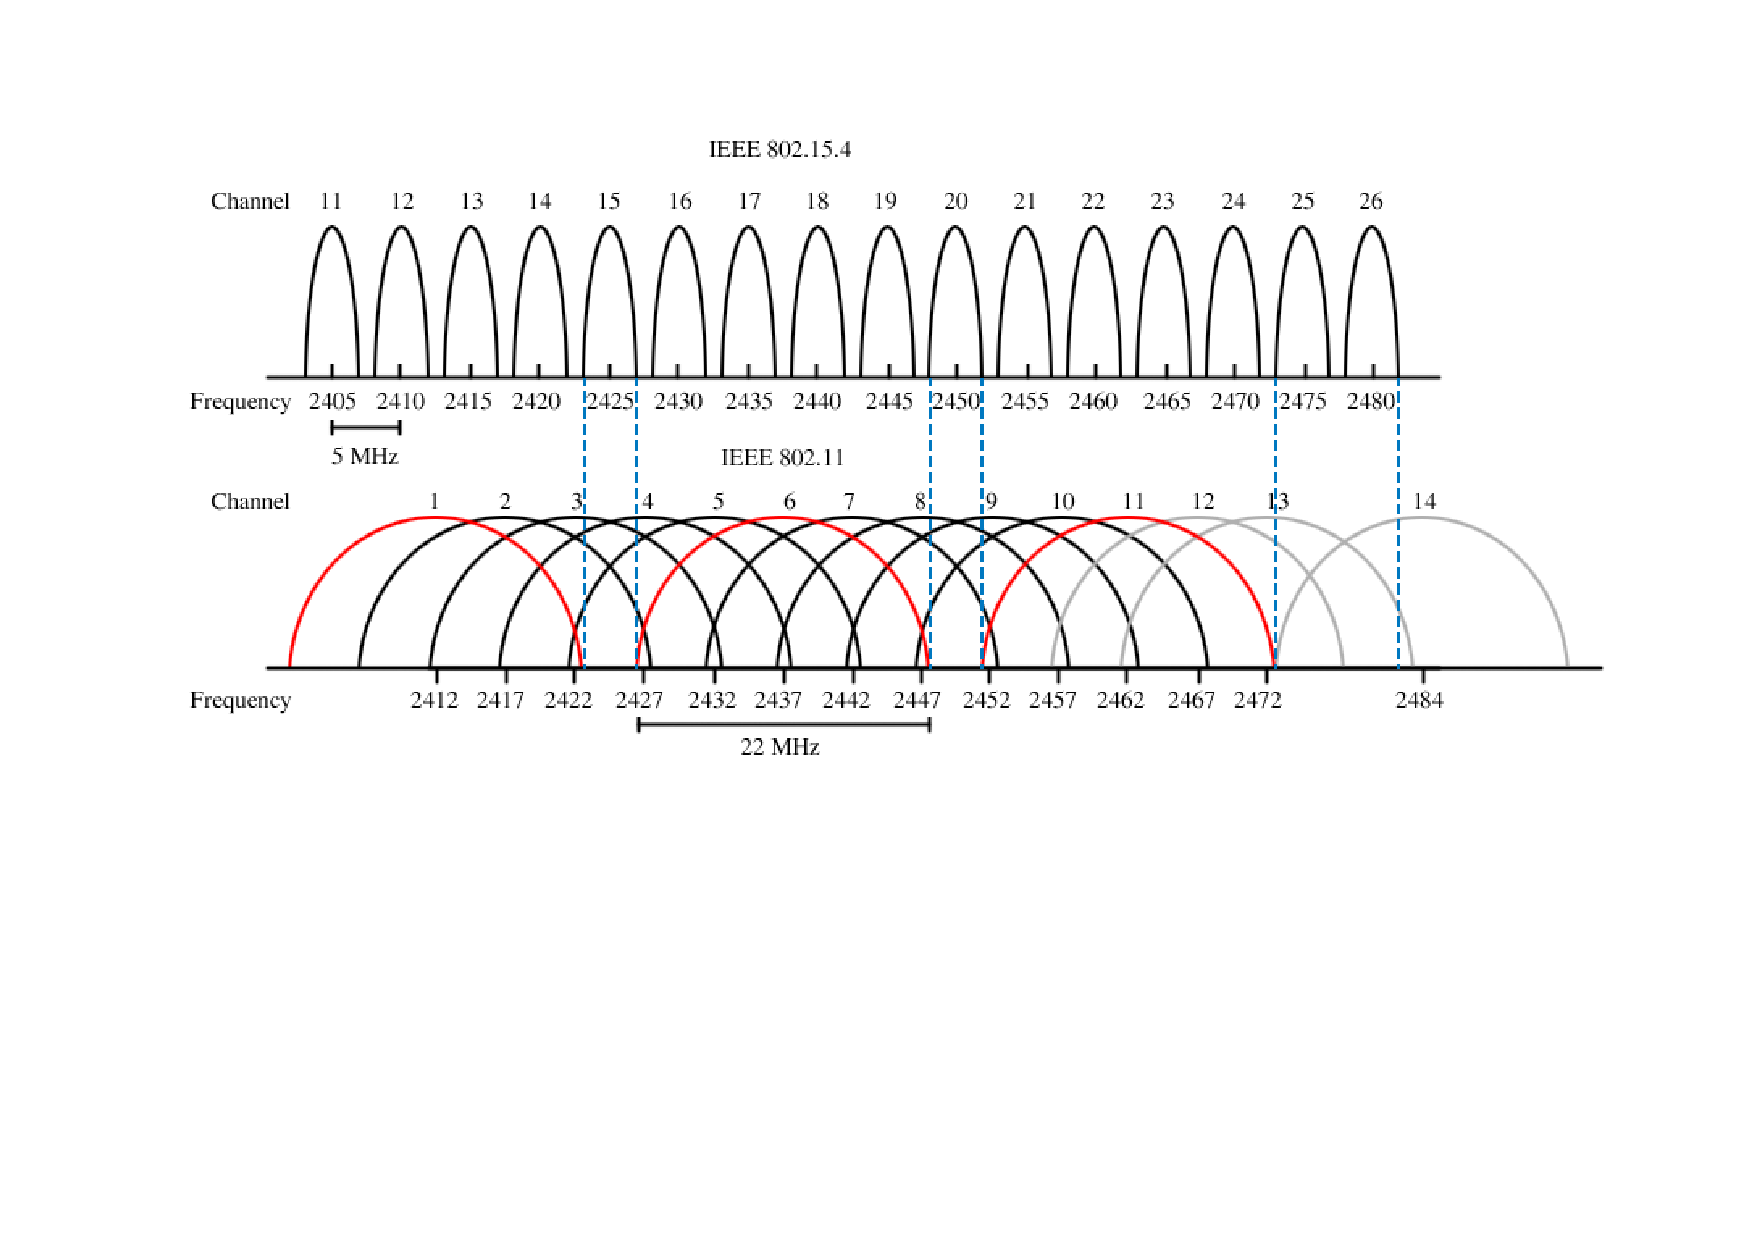
\includegraphics[trim=3cm 8cm 2cm 2cm, clip=true, width=0.45\textwidth]{figures/freqBand.pdf}
%\caption{IEEE 802.15.4 and IEEE 802.11 frequency channels in the 2.4 GHz ISM band}
%\label{fig:freqBand}
%\end{figure}

Upon start up, all nodes are initialised to channel 26 as it does not overlap with Wi-Fi. 
%which does not overlap with the Wi-Fi channels. 
%Channel 15, 20, 25 and 26 do not overlap with Wi-Fi as shown in Figure \ref{fig:freqBand}. 
%However, channel 26 is the selected clear channel based on the channels occupancy tested in three different locations; residential, public area and university (UCL) environments shown in Figure \ref{fig:interference2} where the figure shows only several selected signals. 
The environment condition and the network could be different depending on the location, time and channel occupancy. 
The authors in \cite{homearea} studied the channels reliability in residential areas in several neighbourhoods in comparison to an office (university) environment to show that the spectrum usage may be very different.
%as office environments are typically centrally managed. 
The authors in \cite{oppcast} showed similar results of different spectrum usage when comparing the interference patterns in offices (universities), public areas (shopping malls) and residential environments.
%This is proved in the hardware performance evaluation section by considering different environments in our experiments.
This shows that it is extremely difficult to find a good interference free channel and it varies from one location to another.

%\begin{figure}
%\centering
%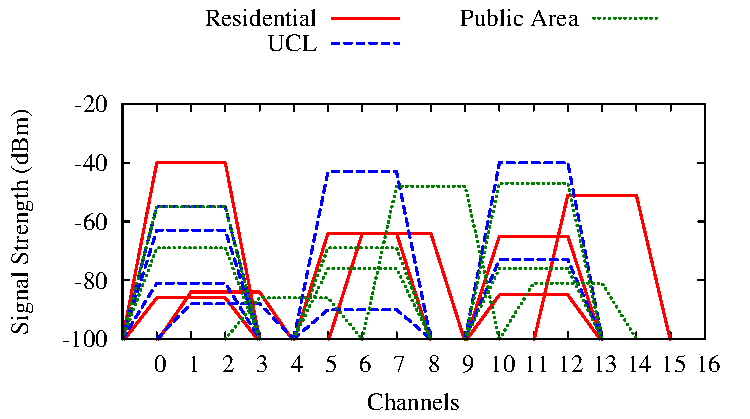
\includegraphics[width=0.45\textwidth]{figures/interference.pdf}
%\caption{Interference level on the channels at different locations}
%\label{fig:interference2}
%\end{figure}

The nodes will only be on the same channel (channel 26) once during the initial setup.
This enables the node to detect and find nearby neighbours that are in range to allow RPL set up mechanism to form the initial optimised topology before channel assignments can take place which improves the tree.
%before it can decides on the best route based on the list of neighbours it can be connected to.
%The usual RPL set up mechanism is used to exchange control messages that are required to form an optimised topology before channel assignments can take place.  
The initial channel should not be used as the transmission channel throughout the runs unless MCRP fails or could not find a better channel in order to not overload the initial channel.
%thus, the change to another interference free or low interference channel. 
It could lead to interference between the nodes competing for transmissions opportunity which is the problem in a single channel network. 
%To ensure reliable communications, two-hops colouring algorithm is used in channel selection to avoid the selected channel from overlapping with the other nearby transmissions.
%Two-hops colouring algorithm ensure reliable communications as the channels do not overlap during transmissions.

\subsubsection{Channel Selection Strategy}
One main advantage of the proposed system is generality. Any algorithm can be used at the LPBR to assign channels. MCRP uses a two-hop colouring algorithm to select a channel to be assigned to a node.
The two-hop colouring algorithm attempts to ensure that nearby nodes do not communicate on the same channel and risk interfering with each other. This enables simultaneous transmissions and allows fair load balancing on the channels. The protocol is inspired by the graph colouring problems \cite{graphColouring}. The core idea is that no node should use the same listening channel as a neighbour or a neighbour of a neighbour (two hops).
%%This allows fair load balancing on the channels and reduces channel interference that could occur when two nearby nodes transmit together on the same channel. 
%%To ensure reliable communications, two-hops colouring algorithm is used in channel selection to avoid the selected channel from overlapping with the other nearby transmissions.

%The nodes used in this experiment have a transmission range of approximately 20-30 metres indoors and 75-100 metres outdoors \cite{telosb-datasheet}. It could be the case that many nodes in a sensor network are in the transmission range of each other and potentially interfered with.

%All nodes are initialised to channel 26 which is the common default channel for Contiki MAC layer since it often has fewer interference problems with Wi-Fi and other sources. The studies in \cite{chrysso, micmac, watteyne} use a set list of whitelisted channels in their experiments and have channel 26 in common.
%However, the initial channel should not be used as the transmission channel throughout the runs (unless all channels check fail) in order to not overload the initial channel, thus, the change to another interference free or low interference channel. It could also lead to interference between the nodes competing for transmissions opportunity which is the problem in a single channel network. 

%Two-hops colouring algorithm ensure reliable communications as the channels do not overlap during transmissions.

%The usual RPL set up mechanism is used to exchange control messages that are required to form an optimised topology before channel assignments can take place. The nodes will only be on the same channel once during the initial setup.
%This enables the node to detect and find nearby neighbours that are in range before it can decides on the best route based on the list of neighbours it can be connected to. 

In the two-hop colouring algorithm, the LPBR chooses a node $N$ to which it will assign a new channel $D$ to listen on.
%The selection is random (from channels 11 to 26) based on the full range available \cite{ieee802.15.4}. 
Instead of checking all or several channels, MCRP chooses a random channel and learns the channel condition from the current run. 
The authors in \cite{energyluca} proposed a spectrum sensing algorithm to decide on the number of channels to be sensed before the channel is selected for transmissions. While it was found that sensing more channels increase the likeliness to find the best channel with less or no interference, it requires higher energy consumption and longer time delay during each check. 
%%%In the studies, three cases were considered where (i) all channels are sense, (ii) the energy consumed (channel conditions) in all channels are known and (iii) in the case where an energy threshold is set in unknown conditions. 
%While the studies showed selecting a channel from several channels check would give better chances of successfully transmit packets, it comes to the cost of energy and require longer period to check several channels.

%Instead of checking all or several channels, MCRP chooses a random channel and learns the channel condition from the current run. 
%The channel condition might vary depending on the location and time, and it could be the case where the same channel has different interference level each time. 
%However, knowing the channel condition does not have any benefit and require all or several channels to be rechecked each time. This consumes a lot of energy during each check. 
MCRP only considers two channels at a time, whether the new channel $D$ has better reception rate than the current channel $C$. By doing so, the channel selection is more spread out (random and fulfil two-hops rule) rather than all nodes trying to use the same best channel.
%The channels that were tested to have severe interference for one node might gives good result for another node depending on the location of the node which might not be within the range of where the channel has severe interference previously. 
%MCRP has its channel quality checking mechanism before it decides on a channel.
The protocol checks the node $N$ neighbours and neighbours of neighbours to see if any of those are currently listening on the selected channel $D$. If any are, a new channel $D$ is randomly chosen from the remaining list of available channels. 
%If the LPBR has knowledge of existing bad channels then those channels can be blacklisted.  
%%%Knowledge of channel interference which is gained by probing can be used to decide that a channel should not be used. If a channel is found then the channel switching protocol is triggered. 
%%???MCRP has its channel quality checking mechanism before it decides on a channel.
If no channel $D$ can be found meeting these conditions, the current channel $C$ is kept. 

The node selection algorithm must only attempt one channel change at a time to ensure probing is done on the correct new channel $D$ and for the node $N$ to finalise the channel to be used before another node attempts a channel change.
The protocol ascertains that the channel change attempt will always result in a message returned to the LPBR either confirming the new channel $D$ or announcing a reversion to the old channel $C$. Until one or other of these happens, no new channel change will be made to ensure that the neighbours are transmitting on the correct channel.

\subsubsection{Channel Switching}

\begin{figure}
\centering
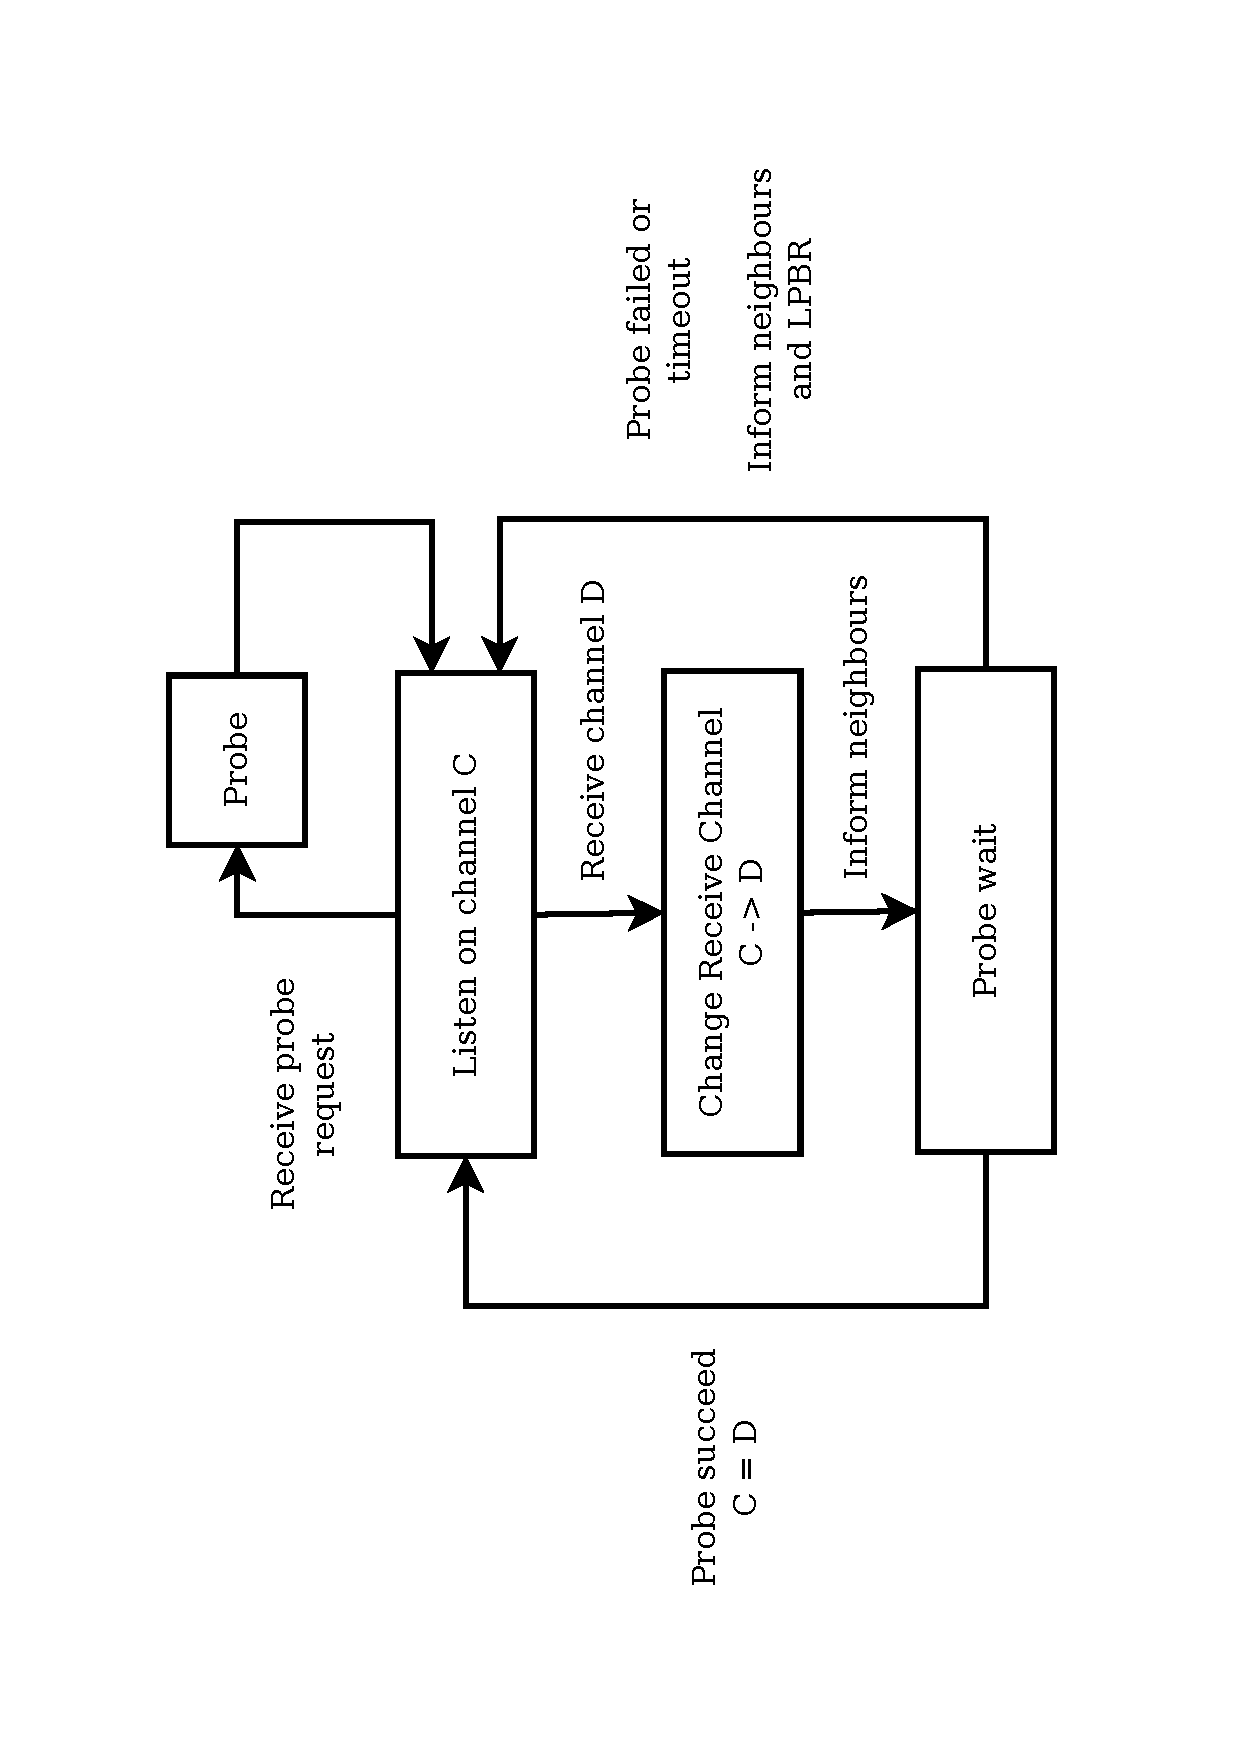
\includegraphics[trim=2cm 2cm 2cm 2cm, clip=true, totalheight=0.36\textheight, angle=270]{figures/channelSwitching.pdf}
\caption{MCRP}
\label{fig_mcrpDiagram}
\end{figure}

%Figure \ref{fig_mcrp} shows the state machine for the channel switching protocol.
As explained in the previous section, a choice of a new channel by the channel selection protocol causes the change channel message to be sent to the appropriate node. Figure \ref{MCRP} shows the steps in the protocol.
Upon receiving the channel change message, the node $N$ stores its current channel $C$ and communicates to all its neighbours the new channel $D$ that it wishes to change to. Those neighbours will update their neighbour tables to ensure that they now send to node $N$ on channel $D$.  The node $N$ begins the channel quality checking process with each neighbour in turn by sending them a probe request. If this process fails for any neighbour then the node reverts to channel $C$. Node $N$ informs its neighbours of the decision. The neighbours will update their neighbour table to transmit on channel $C$. If all channel quality checks succeed, the node $N$ will listens on channel $D$. Node $N$ does not send a confirmation message to the neighbours as it would be redundant since the neighbours already know the node $N$ listening channel. 
%In both cases, LPBR is informed of the channel checking results. LPBR updates the node's channel on its table.   
%In both cases, node $N$ informs its neighbours of the decision to channel $C$ or $D$ and informs the LPBR of the channel checking results. 
%%The channel checking process uses probe packets that might interfere with other transmissions temporarily. However, it is important to emphasise that the network remains fully functional and connected at all stages of this protocol.

\subsubsection{Channel Quality Checking}
Probing is essential to make the channel change decision. It gives a quick overview of the channel condition based on the number of probing messages received. The probe packets might interfere with other transmissions temporarily. However, it is important to emphasise that the network remains fully functional and connected at all stages of this protocol.

Probing is only done between the node $N$ and the tree neighbours. Tree neighbours are the nodes that a node does transmit to through the topology formed by the RPL protocol. The tree neighbour node is selected from the list of available neighbours based on the ability to transmit to the next hop towards the LPBR depending on the RPL. By default, it is decided by using the least expected number of transmission from the node to LPBR. Node neighbours are all nodes that a given node knows it could transmit to. The nodes are within the transmission range of each other.
%In describing the channel quality checking process, it is worth emphasising the distinction between neighbours and tree neighbours.  
Neighbours that are not tree neighbours will not use the node as a route during their transmission thus, there is no need for probing to take place with those neighbours. However, the neighbours still need to know the channel value given that RPL control messages are sent to neighbours directly without using the routes.

The channel quality checking is invoked each time a node $N$ changes channel after receiving a message from the LPBR. 
%The node $N$ changing to channel $D$ informs all neighbours in turn, of the new channel $D$ it will be listening on as described in the previous section. 
It then enters the \emph{Probe Wait} state and begins channel quality checking with each tree neighbour in turn. 
In the \emph{Probe Wait} state, node $N$ sends a \emph{Probe} message to each tree neighbour in turn. The neighbours respond to the message by sending eight packets to $N$ on the new channel $D$. 
The buffer can accommodate eight packets at a time. As the packets might not be sent immediately due to wakes up and collisions, sending more packets would have the risk of being dropped. The authors in \cite{homearea} observed that a short period of time is sufficient to give an overview of the channel condition as increasing the period shows minimal benefit.
The condition of the channel $D$ is further investigated through the number of retransmissions and packet collisions of the probing packets for accuracy of the channel condition. 

If the probing process times out (because of some communication failure) or the number of probe packets received is above a threshold (currently set to 16, including retransmissions and collisions) then node $N$ immediately exits \emph{Probe Wait} state and reverts to channel $C$ its previous channel. 
All neighbours are informed of the change back to channel $C$.
%and the LPBR is informed of the quality check failure with a summary of all probes received.
If, on the other hand, all channel quality checks succeed, the change to channel $D$ becomes permanent for node $N$.
In both cases, the LPBR is informed of the results with a summary of all probes received and the channel.

\subsubsection{Reconnection Strategy}
RPL routing protocol functionality remains the same. RPL control messages are adjusted to support multichannel.
%\cite{routingmetrics, winter2012rpl}.
%RPL topology could change according to the routing metric \cite{routingmetrics} the way the usual RPL would work \cite{winter2012rpl}. 
The nodes can still change the parents as usual as all neighbours are informed of any channel changes.
%for the nodes that are within the transmission range of each other.
%know each other new channels. 
%The neighbours that are not part of the route do not probe the parent when making the channel decision. However, the neighbours are informed of any channel changes.
This enables the topology to be optimised when communication fails and further improved through MCRP as the nodes have knowledge of the listening channels of all other nodes within the range. If a new node tries to join the topology, it sends a RPL control message through all channels as the listening nodes are unlikely to be on the initial channel. The new nodes will start on channel 26.
The listening nodes send a broadcast on the default channel to discover new nodes and send RPL messages through unicast when the neighbours are known to reduce unnecessary transmissions in broadcast on all available channels. New nodes and nodes which fall off the network can now rejoin on many potential channels.

%\subsubsection{Summary}
%This chapter introduces MCRP, a multichannel cross layer routing protocol that jointly optimise the network communications through channel decisions from the application, network and MAC layers. It uses a centralised controller for nodes channel allocation. The channel condition is tested through probing packets during run time as it varies depending on the location, time and usage. By doing so, the nodes would use less interference channels for communications to maximise the packet reception rate. MCRP uses a two-hop colouring strategy to avoid nearby nodes from competing to transmit on the same channel at the same time and internal interference that could occur. In order to allow reconnection and new nodes to join an existing topology, RPL control messages are adjusted to support multichannel. 
\subsection{Simulation Performance Evaluation}

%This chapter presents the evaluation of MCRP. The experiment set ups for Cooja simulation is explained below. In Cooja simulation, interference is introduced. MCRP is evaluated using an end-to-end packet delivery performance metric. The results from the experiments are presented and discussed. 

%///////simulation

%\begin{figure}
%\centering
%\includegraphics[trim=4cm 6cm 2cm 2cm, clip=true, width=0.38\textheight]
%{figures/simulationLayout.pdf}
%\caption{Layout of the simulation nodes}
%\label{fig_simulation}
%\end{figure}

MCRP is evaluated in the Cooja simulated environment. 
%Figure \ref{fig_simulation} shows the layout of the network.
The network consists of 31 nodes which are used to run the simulation where one node is used as the border router node, 16 interference nodes, and 14 duty cycled nodes that act as UDP clients to send packets to LPBR spanning over 20-30 metres between each node. RPL border router is used as LPBR in order to move most processing decisions on a PC as it has more RAM and better processing capabilities than a sensor.
The border router also acts as the root of the tree.

In Cooja simulation, an interference model is used as simulation to allow full control over the test environment and the experiments are repeatable. Although the interference model does not fully mimic the behaviour of the real world interference, it enables MCRP performance to be tested in various conditions when the channel performance is degraded and to have a better understanding of the performance.

%MCRP is evaluated in the Cooja simulated environment with emulation of TMote sky nodes that feature the CC2420 transceiver, a 802.15.4 radio. The nodes run on IPv6, using UDP with standard RPL and 6LoWPAN protocols. Figure \ref{fig_simulation} shows the layout of the network. The network consists of 31 nodes which are used to run the simulation where one node is used as the border router node, 16 interference nodes, and 14 duty cycled nodes that act as UDP clients to send packets to LPBR spanning over 20-30 metres between each node. RPL border router is used as LPBR in order to move most processing decisions on a PC as it has more RAM and better processing capabilities than a sensor. TelosB sensor has limited RAM and ROM of 10K bytes and 48K bytes of flash memory \cite{telosb-datasheet}. By using a border router, this allows channel changing to be decided in real time without draining the memory and battery on a sensor. The border router also acts as the root of the tree.

%\begin{figure}
%\centering
%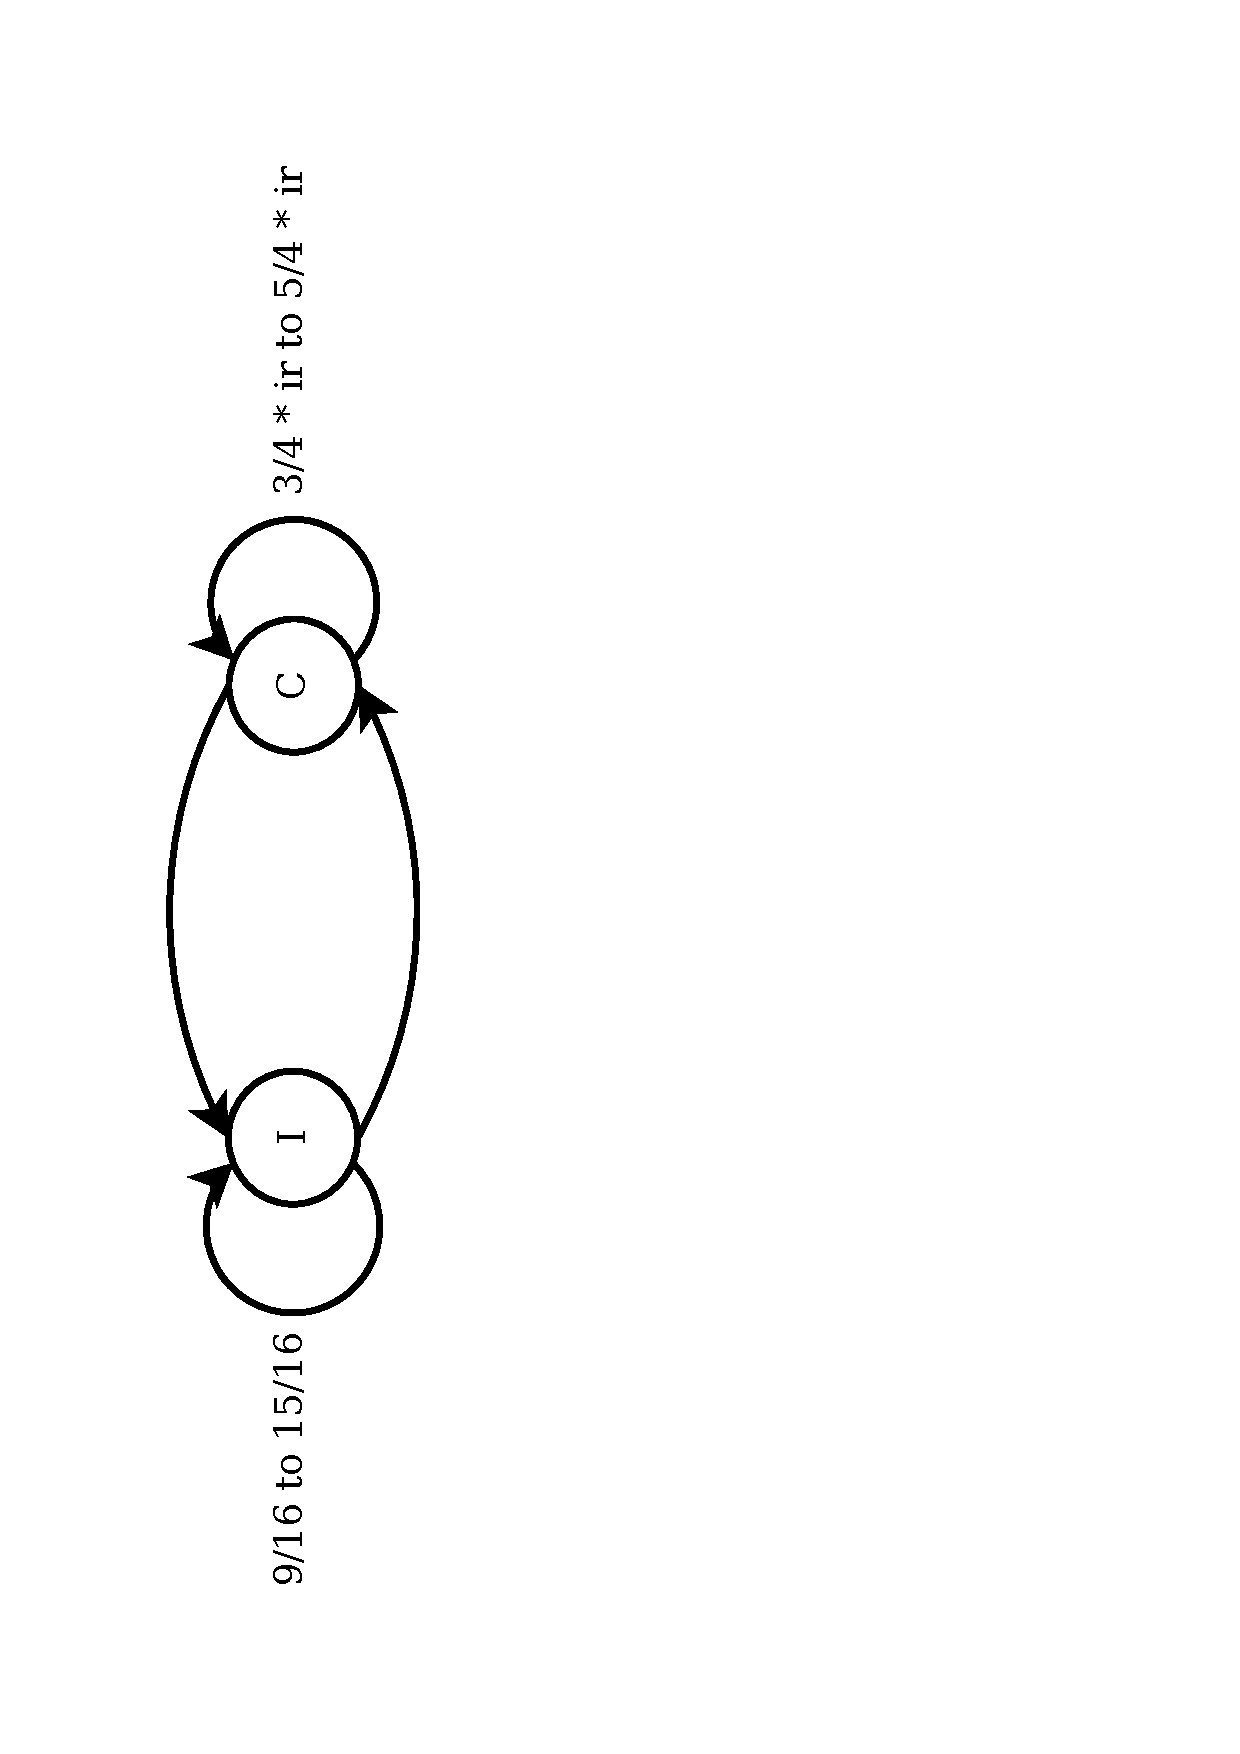
\includegraphics[trim=2cm 2cm 13cm 2cm, clip=true, totalheight=0.36\textheight, angle=270]{figures/interferenceModel2.pdf}
%\caption{Interference model}
%\label{fig_interferenceModel}
%\end{figure}

The controlled interference node generates semi-periodic bursty interference is simulated to resemble a simplified Wi-Fi or Bluetooth transmitter on several channels at random. The interference model proposed in \cite{interferenceModel} is used in the simulation to generate similar packet loss rate to the theoretical and real nodes values given in \cite{radio2009}. The interference has two states, a clear state (C) and an interference state (I). 
In the interference state, the interference node generates packets for a time that is uniformly distributed between $9/16$ seconds and $15/16$ seconds. In the clear state the interferer produces no packets and stays in this state for between $3/4 * \emph{clear\textunderscore time}$ and $5/4 * \emph{clear\textunderscore time}$ where \emph{clear\textunderscore time} refers to the rate of interference (ir). 
%The model is illustrated in Figure \ref{fig_interferenceModel}.
Multiple channels interference is used in the simulation to show the hypothesis that MCRP can help avoid interference. The scenario that is considered is where ContikiMAC with RPL system is subject to interference on its channel after set up has successfully completed so the RPL set up is allowed to complete before interference begins.

The protocol performance in loss over time in the presence of interference is observed. The level of interference used in term of the \textit{clear\_time} is 100\% for no interference, 75\% for mild, 50\% for moderate and 25\% for extreme interference. The percentage represents the ratio of the time the channel is clear for transmission.
Two multiple channels interference scenarios are considered; (i) extreme and no interference rate on 8 channels each and (ii) extreme, moderate, mild and no interference rate on 4 channels each.

The interference channels are randomly chosen from the available 16 channels and the same interference channels and rates are used throughout the experiments. However, channel 26 is kept clear from interference in order to ensure RPL set up is unaffected. In scenario 1, the interference rates are fixed to extreme and no interference to observe the effect it has on the channel changing decisions. In scenario 2, the interference rates are vary to observe how MCRP copes in deciding a channel when there is more interference than scenario 1 but with less interference intensity. 

The simulation runs for a duration of 45-60 minutes to send 210-560 packets. When the nodes are switched on for the first time, all nodes are initialised to channel 26, the default channel for Contiki MAC layer. RPL is allowed five minutes to set up (which is ample time). RPL topology is formed in a minute. The simulation waits for another five minutes to allow trickle timer to double the interval length so that RPL control messages are not being sent frequently. The multichannel protocol is then runs for 25 minutes. In the 15 nodes simulation, the protocol takes 20-25 minutes to run the channel change set up. Another 5 minutes wait time is allowed if retransmissions happen. 
In a single channel simulation, all the nodes are changed to channel 22 after 5 minutes of RPL set up time. This allows RPL to have enough time to discover all nodes to form an optimised topology. The topology formation does not form completely if the interference node interferes from the beginning. 

The interference node starts sending packets to interfere after 3 minutes the system is switched on so that the interference channel is involve in the channel changes decision. It is proven that the protocol tries to avoid changing to the interference channel through time out and probing failures. After 30 minutes, the client nodes will send a normal packet periodically every 30-60 seconds to LPBR. This is done in order to avoid collision of the nodes sending at the same time. 

%\subsection{Simulation Results}
The performance of MCRP is compared against the standard ContikiMAC with RPL and Orchestra to demonstrates MCRP abilities in dealing with external and intra interferences. Orchestra does not support RPL downwards routing due to limited memory in TelosB. It however, support the upwards traffic which is require in the experiments as all traffics are directed upwards towards the LPBR.
MCRP is analysed using an end-to-end packet delivery performance metric, setup overhead, channel switching and reconnection delay in MCRP. The transmission success rate is calculated from the sender to the receiver over multiple hops. 
The simulations are repeated ten times. In all plots, the mean value of the ten simulations is plotted with error bars corresponding to one standard deviation in either deviation to give a measure of repeatability. The plots are of the proportion of received packets (from 0\% to 100\%) against time where the loss is measured over the previous time period.  The x-value is shifted slightly left and right to prevent error bars overlapping.


%%This chapter demonstrates MCRP abilities in dealing with external and internal interferences. MCRP is tested in the simulated environment to study the effect of multichannel to the performance in a controlled environment. MCRP results are compared to the standard single channel ContikiMAC and multichannel Orchestra that implemented TSCH in term of the end-to-end packet delivery. The setup overhead, channel switching and reconnection delay in MCRP are discussed to prove that these values are negligible in the context of WSNs that could run in years while maintaining high throughput.

\subsubsection{Packet Loss Rates}
%%repeatition of what already explained
%The performance obtained in ContikiMAC with RPL (single channel) is compared with MCRP in terms of packet loss rate.
%As described previously, levels of interference used (referred to as \emph{clear\textunderscore time} in \cite{interferenceModel}) vary among 100\% (no interference), 75\% (mild), 50\% (moderate) and 25\% (extreme) where the percentage is the ratio of the time the channel is clear for transmission. All of the tests have a common format: the RPL procedure is allowed to set up without interference in order not to bias subsequent tests.
%Then the interferers begin to operate with a constant level (none, mild, moderate or extreme).

\begin{figure}
\centering
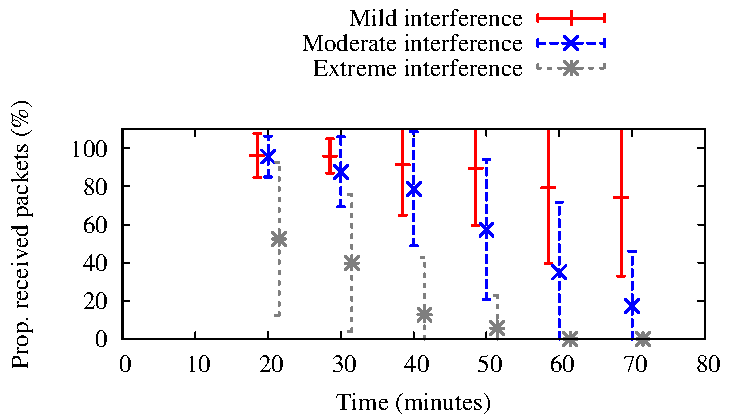
\includegraphics[width=0.45\textwidth]{figures/single_channel.pdf}
\caption{Level of packet loss for mild, moderate and extreme interference levels using single channel}
\label{fig:interference}
\end{figure}

Figure \ref{fig:interference} shows the results in simulation for ContikiMAC with RPL protocol. It can be seen that the level of packet loss varies considerably between experiments (the error bars are always large). It can also be seen that even for mild interference there is considerable loss and this gets worse as time proceeds. In the extreme interference case the loss always goes up until no packets are received. For mild interference the system evolves until it is losing around 20\% of packets but this can increase.

In the single channel, the node does not have enough time to recover from the interference to retransmit and drops all packets. In the extreme interference case, it shows that there are more packets drop over time and it stops receiving packets as it doesn't have enough buffer to store the incoming packet and the channel becomes congested. However, as the interference rate increases (less interference), the single channel performance improves as it has more time to recover.

%%The results from the single channel with interference is compared with the multichannel with the same interference rate of 75\% (mild), 50\% (moderate) and 25\% (extreme). The test is done to evaluate MCRP behaviour in different interference rate and to compare the result with a single channel case. 

%Figure \ref{fig:sminterference} shows the averaged results from ten runs that were done. It can be observed that during high and moderate interference, if LPBR tries to send a channel change value that is the same channel as the interference, the request will either timed out or if it succeeds, the probing messages received are less than a threshold that allows for the node to change its listening channel to the new channel. This is as expected as MCRP checks the channel each time before deciding on the new channel to avoid interference channel. By doing this, it ensure that the node's listening channel is a good channel. This enable the use of all available channels without blacklisting any channel until it is sure that it is a bad channel through the probing process. The channel quality table is built at the LPBR that over time can be used to learn good and bad channels based on several probing processes. MCRP avoids the interference channel which as a result, resulted in less loss than in a single channel case. 

%In the single channel, the node does not have enough time to recover from the interference to retransmit and drops all packets. Figure \ref{fig:extreme} shows that there are more packets drop over time and it stops receiving packets as it doesn't have enough buffer to store the incoming packet and the channel becomes congested. However, as the interference rate increases (less interference), the single channel performance improves as it has more time to recover.

%In the mild interference case, all probing messages are received even though there is interference in that channel. This means that the channel can be used for transmission. As the interference rate is mild, all packets are received. This is also the case with a single channel. The interference does not affect the transmissions as the interference is not frequent enough. The node has enough time to recover from the interference through retransmissions. However, the interference would slightly effect the packet transmission over time. The channel change processes should run periodically to avoid this from happening.

\begin{figure}
\centering
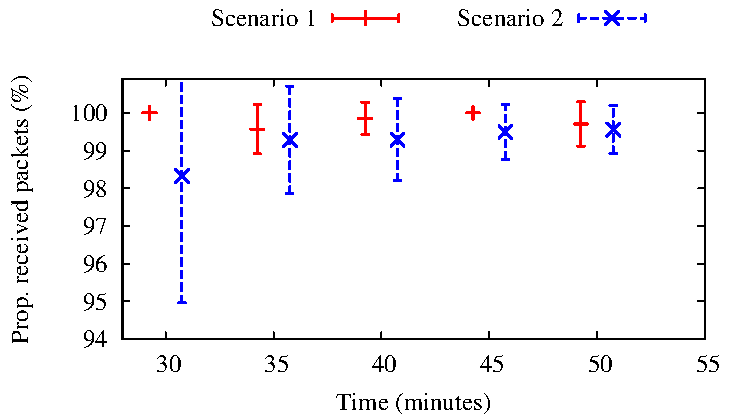
\includegraphics[width=0.45\textwidth]{figures/multi_channel.pdf}
\caption{Level of packet loss for scenario 1 and scenario 2 using multichannel}
\label{fig:multi_interference}
\end{figure}

To evaluate MCRP capabilities to cope with interference from many sources, thus channels, and to compare to a single channel, two interference scenarios are considered.
In scenario 1 half the channels (including the original channel) have no
interference at all and half the channels have extreme interference.
In scenario 2, four channels (including the original channel) have no
interference, four have mild, four moderate and four extreme interference.
Figure \ref{fig:multi_interference} shows multichannel results for these
two scenarios. In scenario 1 the protocol performs extremely well, the packet loss is near zero and the protocol successfully detects channels with interference.
Scenario 2 has similar results as in scenario 1. The protocol does well at reducing the effects of interference and could detect moderate and mild interference.
%Figure \ref{fig:sminterference} shows the averaged results from ten runs that were done. It can be observed that during high and moderate interference, if LPBR tries to send a channel change value that is the same channel as the interference, the request will either timed out or if it succeeds, the probing messages received are less than a threshold that allows for the node to change its listening channel to the new channel. This is as expected as MCRP checks the channel each time before deciding on the new channel to avoid interference channel. By doing this, it ensure that the node's listening channel is a good channel. This enable the use of all available channels without blacklisting any channel until it is sure that it is a bad channel through the probing process. The channel quality table is built at the LPBR that over time can be used to learn good and bad channels based on several probing processes. 
MCRP avoids the interference channel which as a result, resulted in less loss than in a single channel case. 

In scenario 2 where there are mild interference channels, most of the probing messages on those channels are received. This means that the channels can be used for transmission. This is also the case with a single channel. The interference does not affect the transmissions as the interference is not frequent enough. The node has enough time to recover from the interference through retransmissions. However, the interference would slightly effect the packet transmission over time. 
%The channel change processes should run periodically to avoid this from happening.

\begin{figure}
\centering
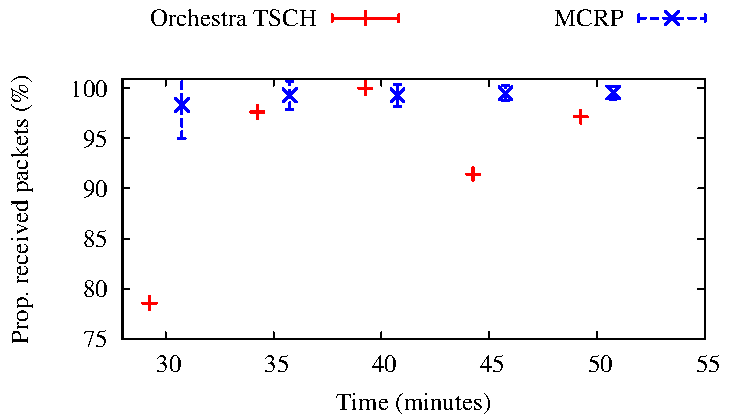
\includegraphics[width=0.45\textwidth]{figures/tsch1.pdf}
\caption{Level of packet loss on testbed for MCRP and Orchestra}
\label{fig:orchestra_sim}
\end{figure}

To prove that MCRP also performs better than not only single channel protocol, MCRP is compared against Orchestra. In the experiment, Orchesta uses channel hopping on all 16 channels. Figure \ref{fig:orchestra_sim} shows the result from scenario 2 on both MCRP and Orchestra. Orchestra has a low packet loss showing around 90-100\% received packet as it hops on all channels which includes the channels that have higher interference. In comparison, MCRP selects certain channels to change into after checking the channels condition which gives MCRP nearly zero packet loss. Orchestra shows good result as it hops to another channel in the next iteration which allows it to move from the interference channel faster to be able to keep the loss rate to a minimum. While Orchestra has high proportion of received packets, MCRP shows near 100\% packet reception. Orchestra shows no deviation as the channel values are fixed for each iteration thus giving the same results each time unlike MCRP where the channels are selected at random before it is used.

%In MiCMAC \cite{micmac}, it is stated that MiCMAC has a transmission success rate of 99\% when using four channels. However, when more than four channels are used (8 or 16 channels), MiCMAC performance degrades to approximately 88\% (16 channels) due to interference channels. The interference model that MiCMAC uses is different than in this experiment. They compare the result with Chrysso where Chrysso has a transmission success rate of approximately 88\% for 4 and 8 channels and suffers greatly in the case of 16 channels with 60\% success rate.
%MCRP on the other hand, shows greatly reduced loss rate with any number of channels at approximately 99\%.

\subsubsection{Setup Overhead}
Obviously the system of changing channels and probing to see if a channel is free of interference introduces a certain amount of overhead into
the protocol. This takes the form of (a) extra messages passed and (b) extra time taken to set up. Default RPL on ContikiMAC for the topology considered in these experiments completed its set up using 276 packets. MCRP, the multi-channel protocol completed its set up in 716 packets, that is an overhead of 440 packets on top of RPL. 
This overhead comes from the channel changing messages to nodes and neighbours, probing messages, channel confirmation messages and acknowledgement packets which are required to ensure a thorough channel change decision.
However, it is worth mentioning that this is a one-off cost. This represents (in this experimental set up) approximately one hour of extra packets in the situation of a deployment that is meant to work for weeks or months.  In terms of set up time, the protocol begins to change channels only when the RPL set up process is complete (or at least stabilises). The set up time is 1154 seconds beyond the RPL set up time of 286 seconds. However, it should be noted that, in fact, the system remains fully functional and capable of sending packets during the set up so this set up overhead does not matter to data transmission.
Therefore it can be concluded that data sending costs (extra packets) of set up are negligible in the context of a deployment that will last more than a day. The extra set up time is also negligible within this context and furthermore does not degrade performance of the network during this set up phase.

\subsubsection{Channel Switching Delay}
Each node has different listening and transmitting channels. When the node is awake, it waits for incoming packets on its listening channel. If the node has a packet to send, it will switch to the next hop listening channel based on the channel information from the neighbour table. The channel switching takes at most 100$\mu$ to switch to the transmission channel. This delay is negligible in the low packet rate WSN. MCRP ContikiMAC uses a transmission phase-lock where the transmission node knows the receiver wake up phase. The node starts transmitting just before the receiver is expected to be awake. The channel switching happens shortly before the receiver is ready to receive the packets, thus the time taken in channel switching does not affect the packet reception.
The node goes back to sleep once the transmission has succeeded or reached the maximum number of retransmissions (packet loss). In the next iteration, the node is reset and wakes up on its listening channel. 

The channel reset is done in these cases: (i) the queue buffer is empty, (ii) before sending the next packet from the queue buffer, and (iii) the last packet in the queue buffer has been sent. This reset is done to avoid any delay in packet reception that could happen when the node is awake.

\subsubsection{MCRP Reconnection}

\begin{figure}
\centering
\subfigure[Initial tree]{\label{fig:r1}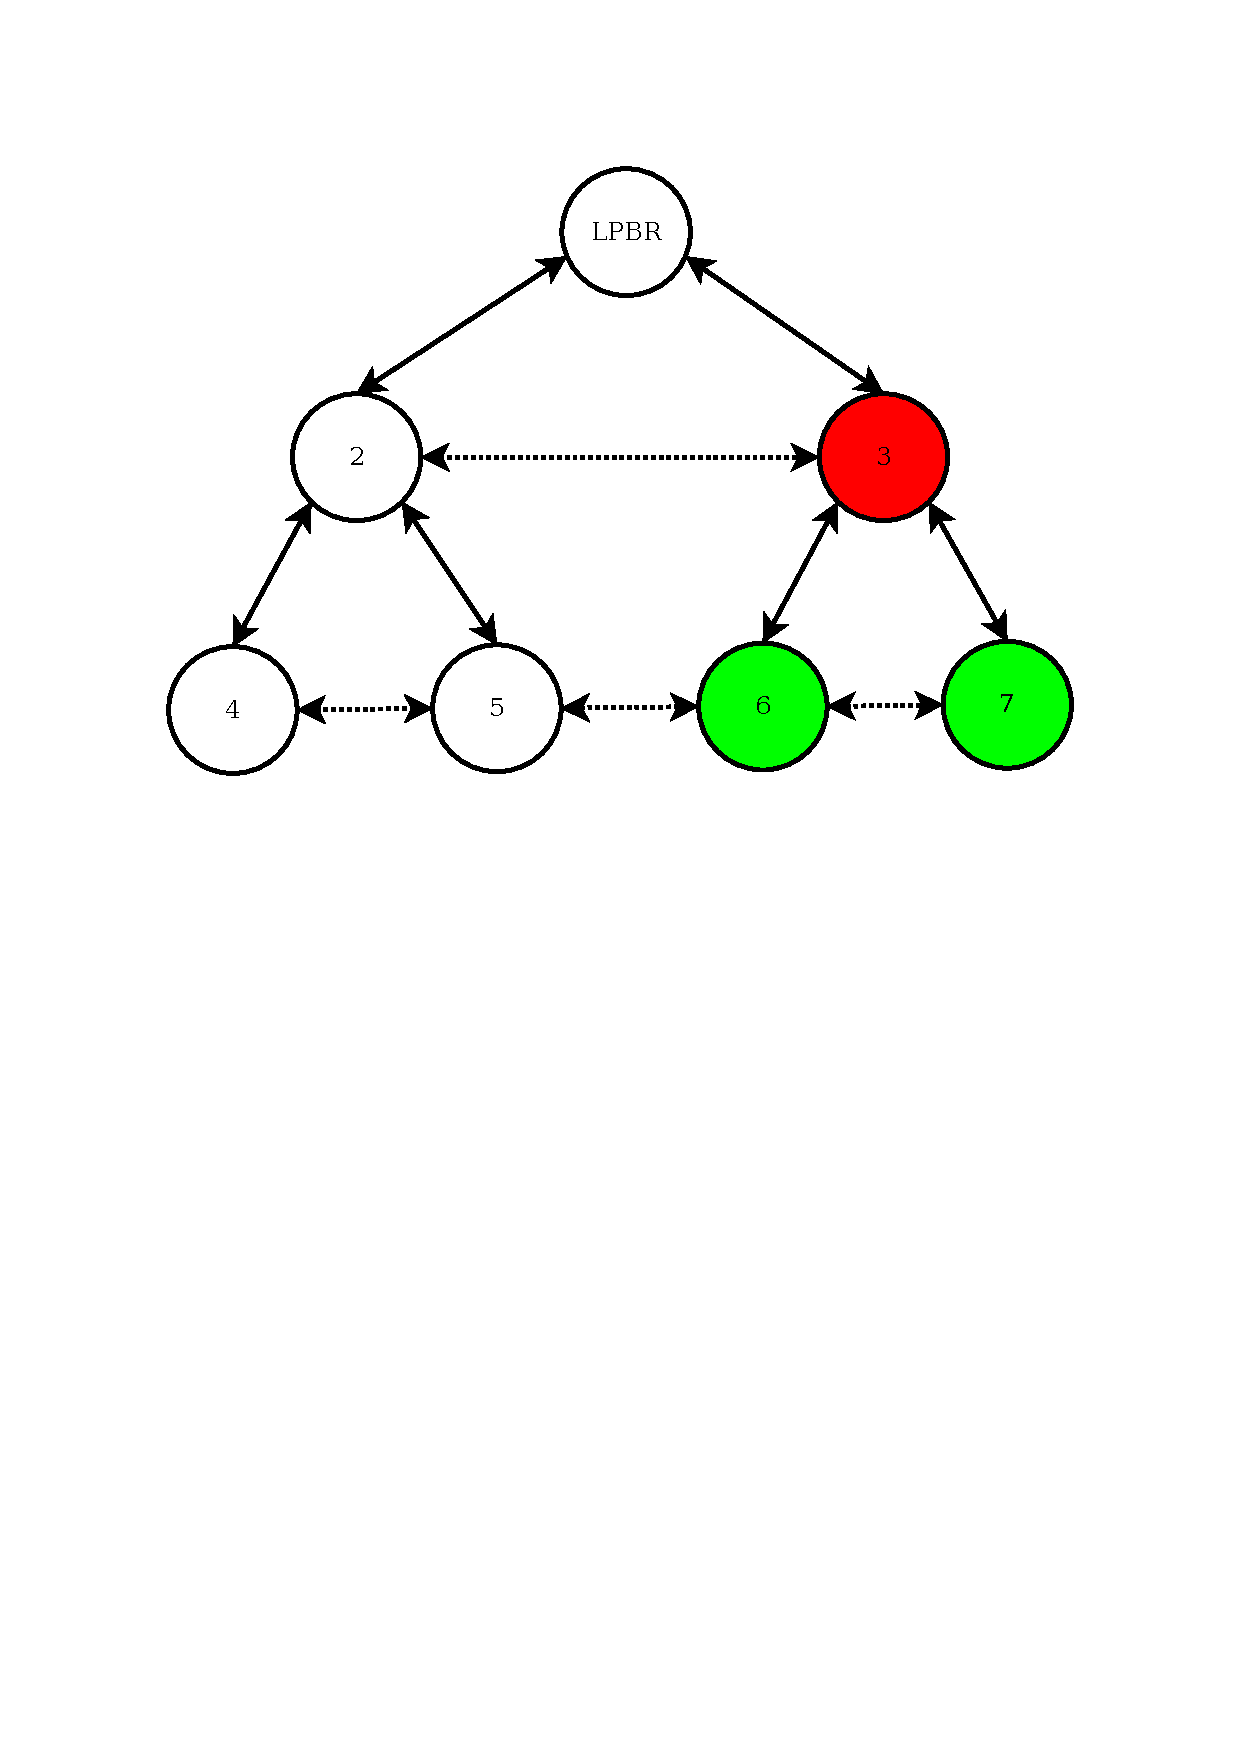
\includegraphics[trim=2cm 16cm 2cm 2cm, clip=true, totalheight=0.12\textheight]
{figures/reconnection1.pdf}}        
\hfill        
\subfigure[Reconstructed tree when node 3 is undetected]{\label{fig:r2}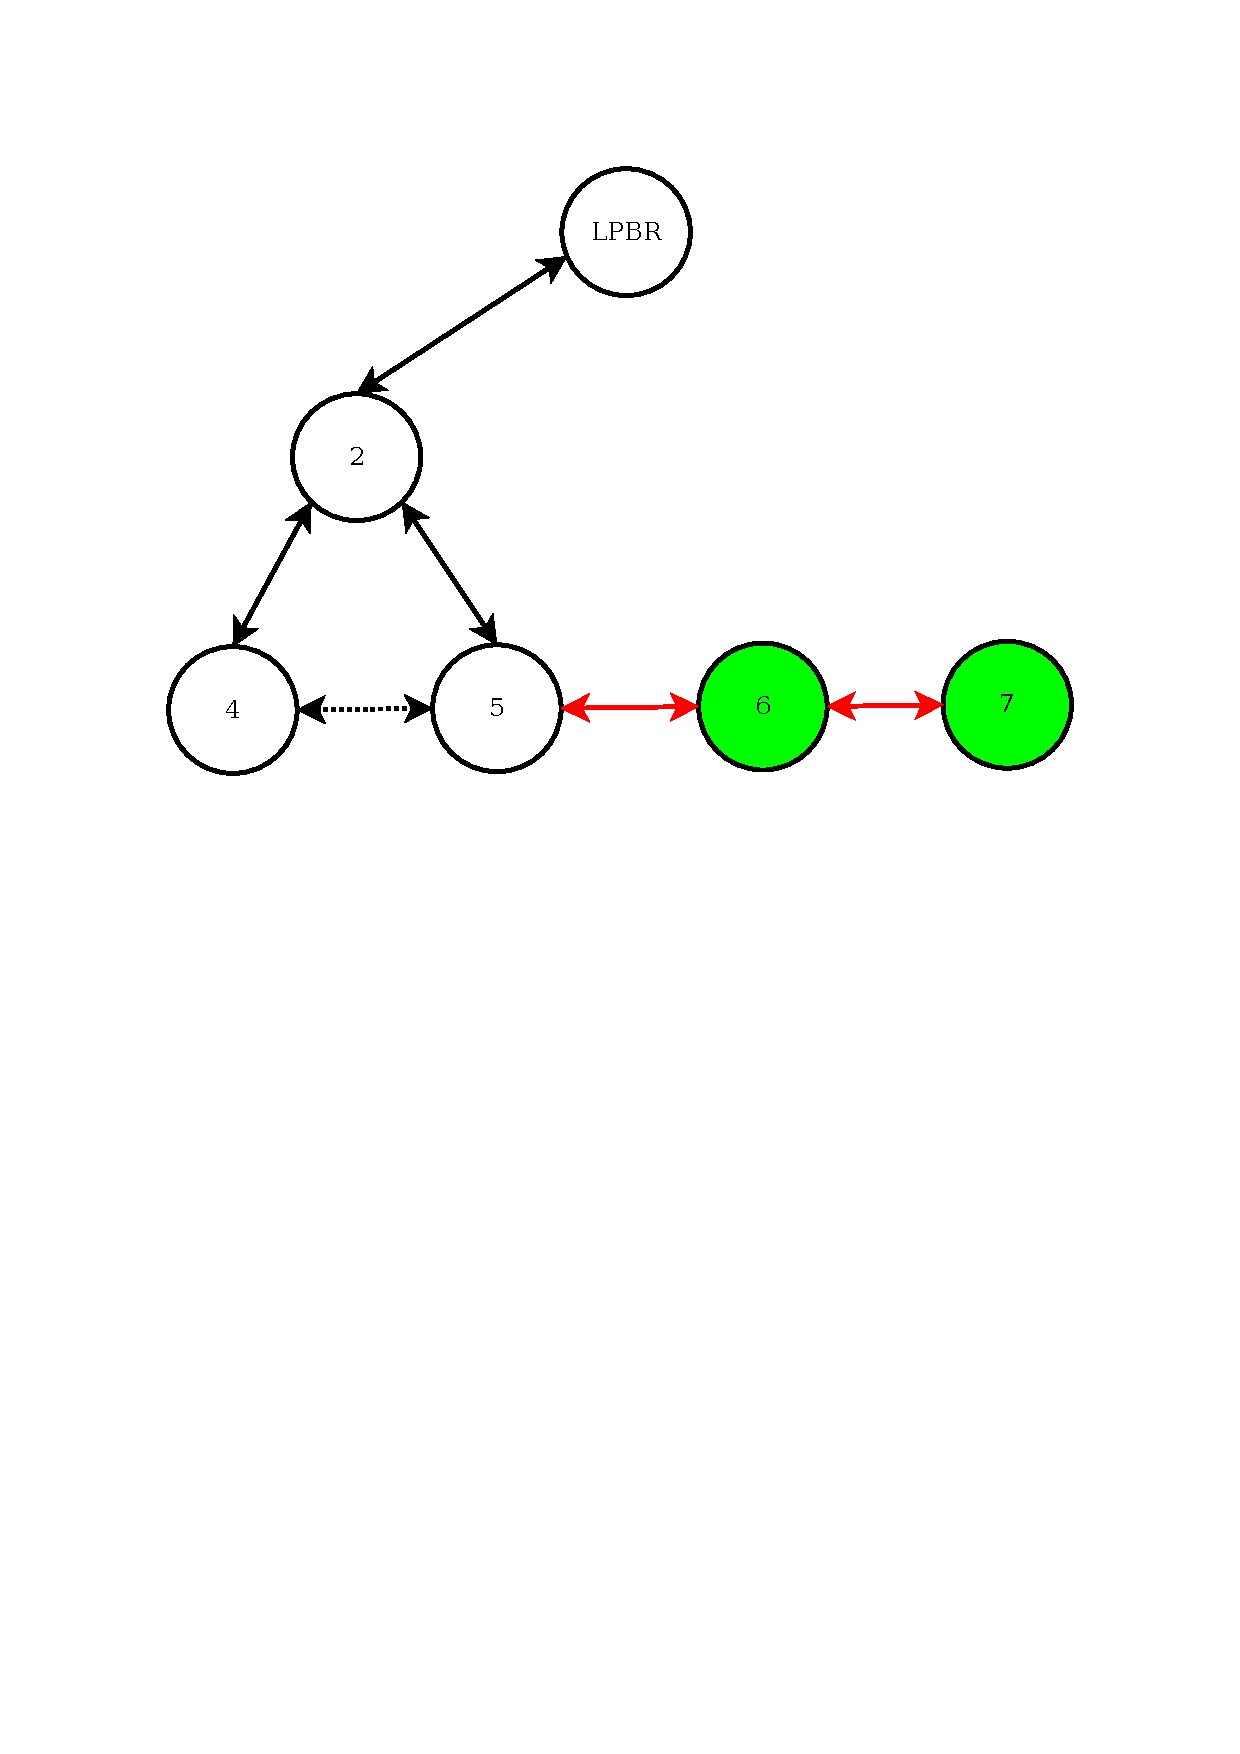
\includegraphics[trim=2cm 16cm 2cm 2cm, clip=true, totalheight=0.12\textheight]
{figures/reconnection2.pdf}}
\caption{A simple simulation layout to test the tree reconnection}
\label{fig:reconnectionLayout}
\end{figure}

\begin{figure}
\centering
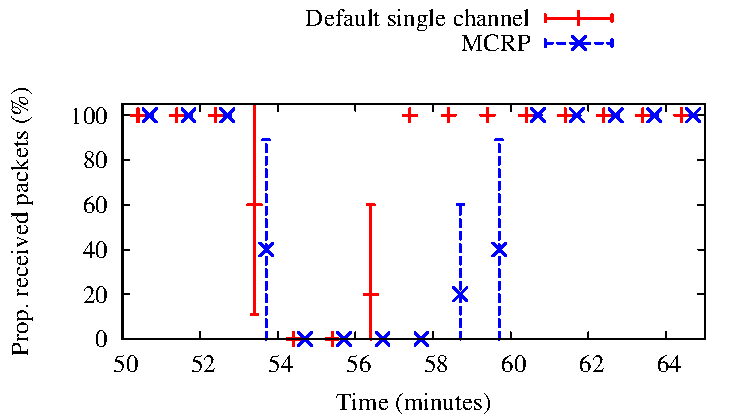
\includegraphics[width=0.45\textwidth]{figures/reconnect.pdf}
\caption{Reconnection time taken for MCRP and single channel}
\label{fig:reconnection}
\end{figure}

%In this thesis, the nodes are assumed to be static. The location and the number of nodes are constant. However, for future improvement, MCRP needs to be able to adapt to mobile network and additional nodes after the initial run time. MCRP results in detecting and adjusting the routes are compared with a single case scenario. 

Figure \ref{fig:reconnectionLayout} shows the experimental setup to test MCRP reconnection in term of the time taken to detect and adjust the routes when a node fails (run out of battery or cannot be detected). There is no external interference introduced to ensure an accurate convergence time of the topology. The dotted lines represent potential paths and the solid lines are the selected paths. The result from MCRP is compared to a single case scenario with the same setup.
%Each node sends 25 packets before a node becomes dysfunctional.
In the figure, node 3 is disabled after 53-54 minutes (25 packets are sent and received). Node 6 and 7 route through node 3 to the LPBR. When node 3 is dropped, node 6 and 7 have to find another route which is through node 5 and 2 to get to the LPBR. The time taken for the nodes to reconfigure the routes and the number of packet loss are showed in Figure \ref{fig:reconnection}. 

In MCRP, it took between 5-7 minutes before node 6 and 7 discover and reconnect with the tree to proceed with the transmission. Single channel however, was slightly quicker, taken 3-5 minutes. The reason for this is MCRP control packets are sent on several channels, thus it would take slightly longer to be able to reach all nearby nodes that might be on different listening channels. A single channel on the other hand, could send a broadcast to the nodes which help to reduce the time taken during the topology reconnection.
The reconnection time in MCRP is acceptable as MCRP shows high packet reception once the route is discovered in interference cases.

Comparing to Orchestra, Orchestra is a synchronous protocol. It has a dedicated slot and periodic schedule for RPL signalling which means it detects the failed node quicker unlike in MCRP and default single channel asynchronous protocols. The results from the Orchestra simulation shows that as Orchestra has a slot checking the nodes every minute, it is able to reconnect the nodes without having any packet loss. The disadvantages of Orchestra are, the nodes are listening on the same channel during the broadcast which the known channel is prone to attack. Also, even though Orchestra introduces priority to the traffic, RPL traffic is sent frequently at every period if there is no other higher priority traffic. Trickle timer that is used by the default RPL has the advantage of reducing the number of redundant control packets by doubling the waiting time for the control packets. Orchestra detects failed node quicker at the cost of frequent control packets that are redundant in a stable topology which increases the use of bandwidth and nodes energy consumption.

%/////

%This chapter demonstrates MCRP abilities in dealing with external and internal interferences. MCRP is tested in the simulated environment to study the effect of multichannel to the performance in a controlled environment. MCRP results are compared to the standard single channel ContikiMAC and multichannel Orchestra that implemented TSCH in term of the end-to-end packet delivery. The setup overhead, channel switching and reconnection delay in MCRP are discussed to prove that these values are negligible in the context of WSNs that could run in years while maintaining high throughput.
\subsection{Hardware Performance Evaluation}

%This chapter presents the performance evaluation of MCRP on the hardware and testbed. The experiment set ups for TelosB and FlockLab \cite{flocklab} testbed are explained below. Similar to the simulation, MCRP is evaluated using an end-to-end packet delivery performance metric. The results are presented and analysed. 

The real hardware experiments provide the ability to validate MCRP performance in the real wireless channel environments unlike simulation. However, the network's behaviours are complicated to examine as the experiments are not repeatable. The environment condition and the network could be different at each iteration depending on the location, time and channels occupancy. The authors in \cite{homearea} compared the channel occupancy in the office and home environments which potentially can have distinct channel usage. This affects the results differently as the channel conditions could have drastic changes during the run time in the residential environments than in the office environments.

The experiments of MCRP were taken place in both residential and university environments with the same experimental setup.
The results are compared to the single channel case to analyse the MCRP performance in various environments.
A small number of nodes are used in order to confirm that MCRP is working. 
The network consists of 10 nodes; 1 border router and 9 duty cycled nodes. The nodes are placed within at least 1 node's range (approximately 15-80 cm); at the power level of 2 which should have nearly 100\% packet reception given that there is no interference at the range of around 20 cm. 
%The network consists of 7 nodes; 1 border router and 6 duty cycled nodes. The nodes are placed within at least 1 node's range (approximately 15-80 cm); at the power level of 2 which should have nearly 100\% packet reception given that there is no interference at the range of around 20 cm. 
%The reason for this is simplicity to be able to repeat the experiments easily. 
It is done to have a smaller scale of network where all nodes would have the same interference source that affects the nodes. Also, to ensure that the nodes would have at least one hop to the sink to fulfil MCRP criteria in changing channel processes. This experiment can be duplicated to cover a larger scale as the radio has the range that could span over 20-30 metres. 

%\begin{figure}
%\centering
%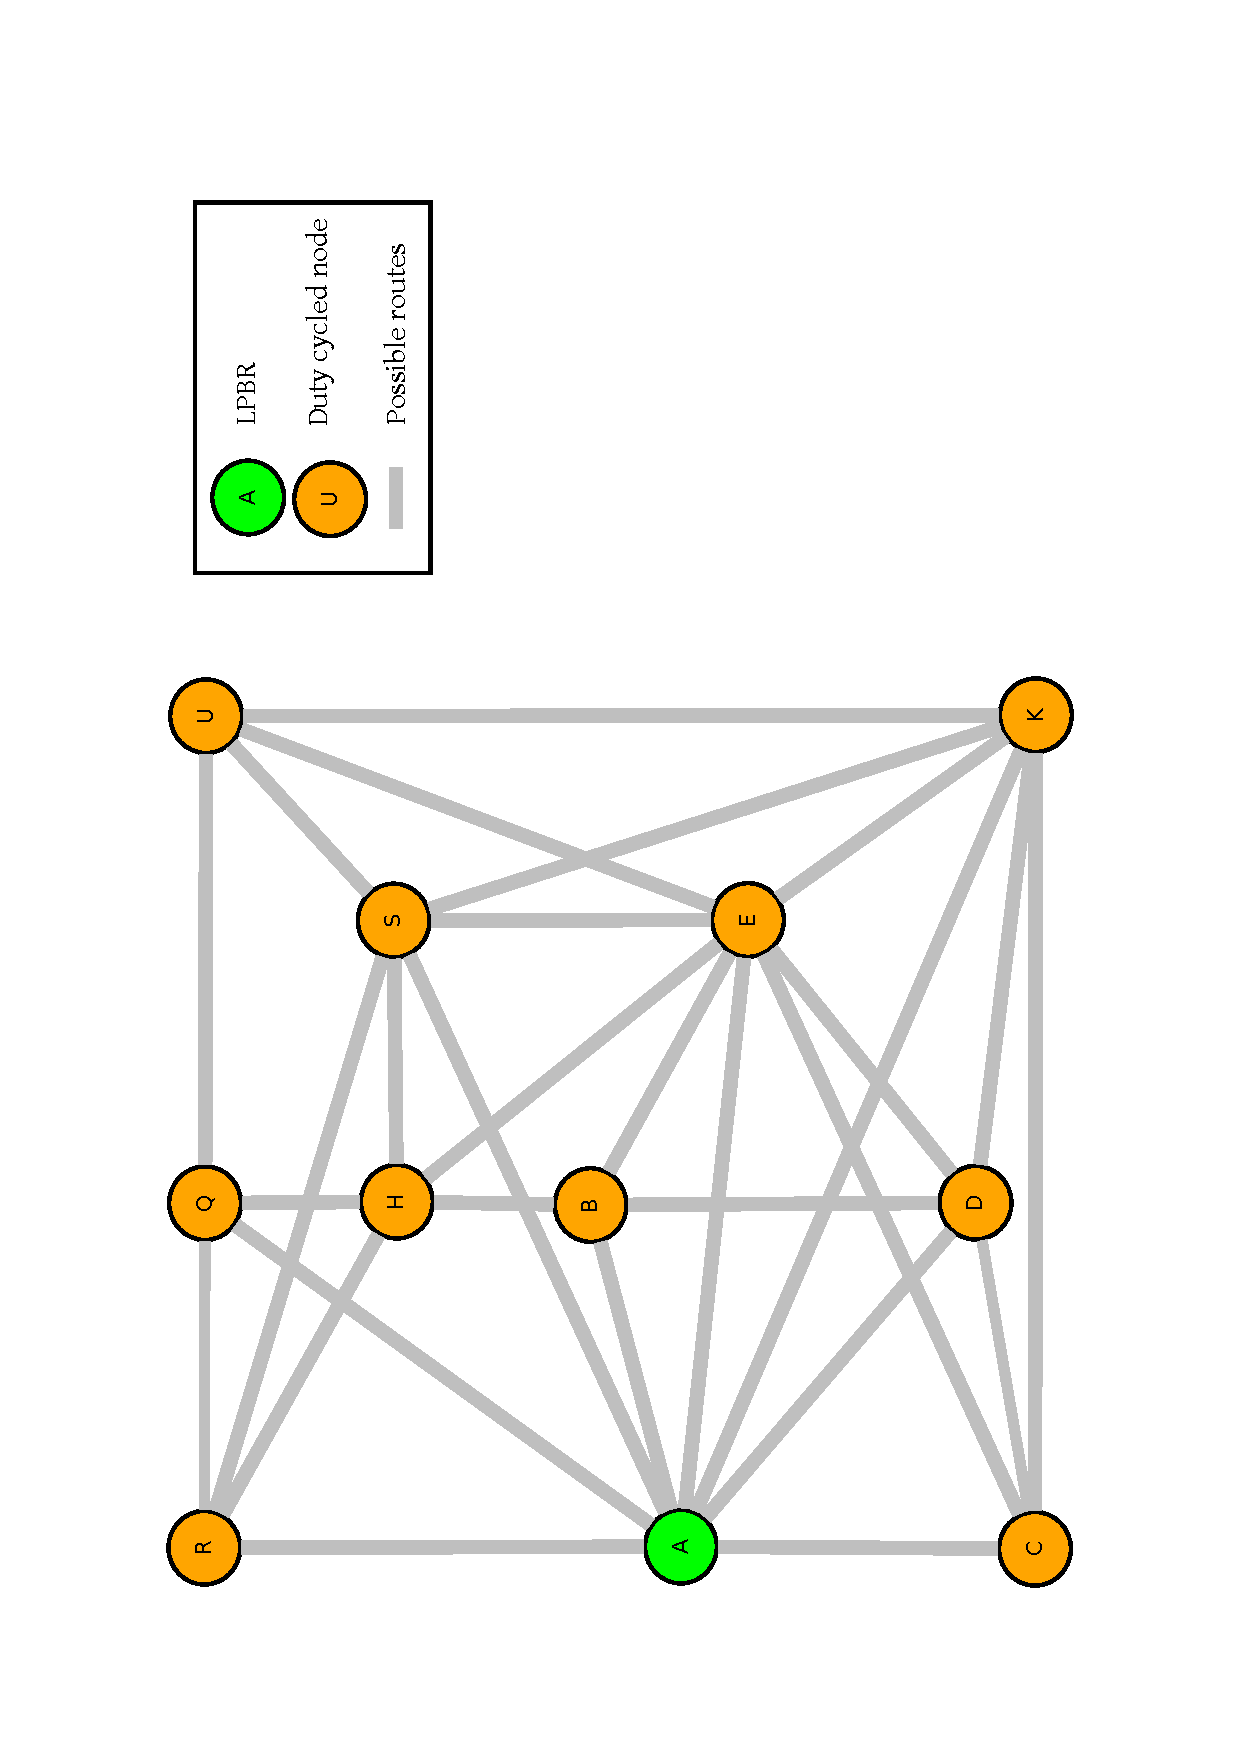
\includegraphics[trim=2cm 2cm 2cm 2cm, clip=true, %totalheight=0.35\textheight, angle=270]{figures/10nodesLayout.pdf}
%\caption{Layout of the real nodes}
%\label{fig_hardwareLayout}
%\end{figure}

The MCRP experiment is run for a duration of 2 hours to send 450 packets, which is 50 packets per node, sending 1 packet per minute for each node. As the nodes are switched on at nearly the same time, RPL is allowed five minutes to set up. MCRP is run for 45 minutes for the channel changes processes. The nodes wait for the MCRP process timer to time out before the nodes can send normal packets. 
%The experiment is then repeated with 11 nodes (1 LPBR, 10 duty cycled nodes) to study the effect that MCRP has with the increased number of nodes. 
The experiments are repeated ten times each. %Figure \ref{fig_hardwareLayout} shows the layout of the nodes and the possible routes that the nodes could choose to get to the LPBR.

%\subsection{Hardware Results}

%%repeatition
%MCRP is compared against the single channel ContikiMAC with RPL.
%Similar to the simulation, the end-to-end packet delivery is used as the performance metric. The proportion of received packets from the sender over multiple hops is plotted with the error bars corresponding to one standard deviation in either deviation to give a measure of repeatability. The values on the x-axis are shifted slightly to avoid overlapping error bars. The experiments of the hardware and testbed are repeated ten times.

Similar to the simulation, the end-to-end packet delivery is used as the performance metric.
The interference could occupy and affect the channels differently at each run. Unlike in the simulation, the RPL tree formation set up is affected by the interference during initialisation. The network could be formed differently at each iteration.

As the nodes are at a close range to the LPBR, some of the nodes could not run the MCRP processes as MCRP requires at least one hop to be able to check the channel condition. However, several nodes were able to run MCRP processes. The tree topology formed differently each time depending on the radio coverage and interference level which affect the RPL ETX value for next hop selection. By increasing the number of nodes and area coverage, it increases the chances that the nodes would have routes to or from which enables MCRP to be executed.

%\begin{figure}
%\centering
%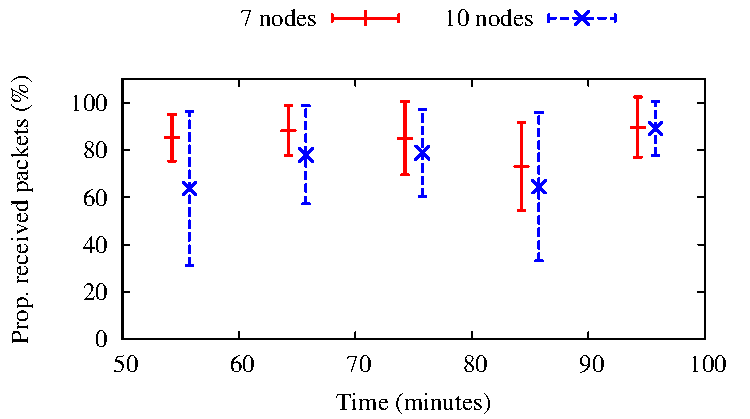
\includegraphics[width=0.45\textwidth]{figures/allNodes.pdf}
%\caption{Real world: Level of packet loss for MCRP}
%\label{fig:hardware}
%\end{figure}

\begin{figure}
\centering
\subfigure[Residential environment]
{\label{fig:hardwareHome}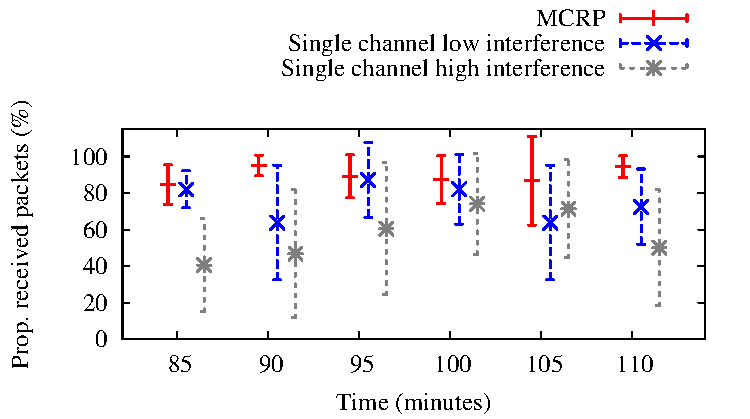
\includegraphics[width=0.45\textwidth]{figures/home.pdf}}
\subfigure[Office environment (UCL)]
{\label{fig:hardwareUCL}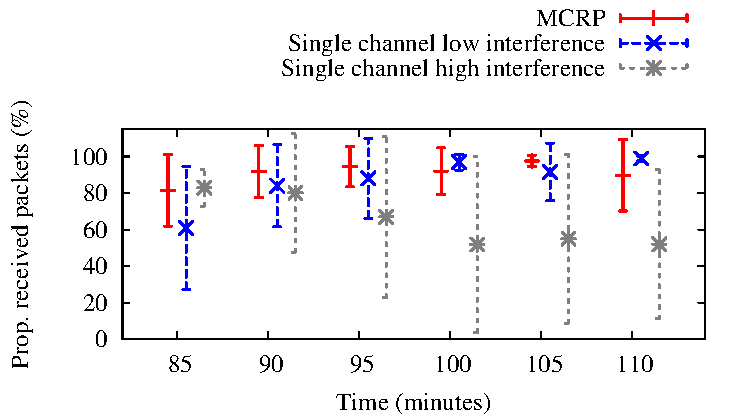
\includegraphics[width=0.45\textwidth]{figures/ucl.pdf}}
\caption{Real world: Level of packet loss for MCRP and single channel}
\label{fig:hardware}
\end{figure}

Figure \ref{fig:hardware} show the results from the experiment in residential and office environments for MCRP compared to a single channel in low and high interference. It can be seen that in both graphs, the number of MCRP received packets vary from approximately 60\% to nearly 100\%. This is because MCRP could hardly find a clear channel for transmissions unlike in the simulation results that show high reception values.
In the single channel case, it can be seen that the results are acceptable in the low interference case. It shows better result in the office environment than in the residential environment as the spectrum usage in the office environment is typically centrally managed. However, both graphs show smaller number of packet reception rate in the extreme interference case compared to the other cases. This shows that MCRP has more advantage than a single channel in extreme interference regardless of the locations. The results are fairly acceptable due to the unpredicted interference occupancy in the 2.4 Ghz frequency band.


%However, in both results, the number of packets loss decreases over time except for at minute 85 before it stabilises again. The reason for this is, the control packets are being sent at the same time (due to trickle timer which enables control packets not to be sent frequently) which resulted in many normal packets to be dropped and lost.

%\begin{figure}
%\centering
%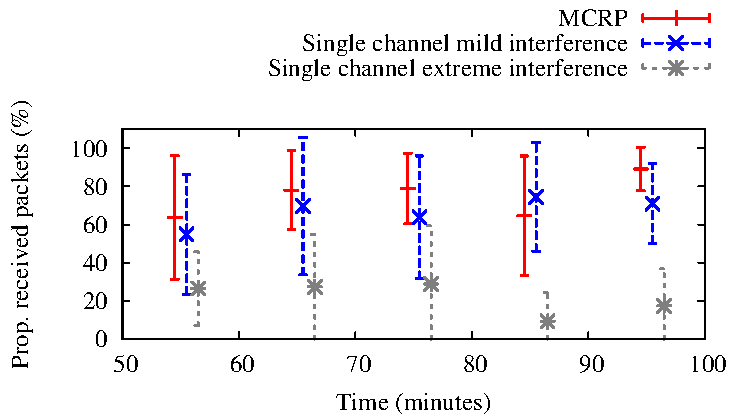
\includegraphics[width=0.45\textwidth]{figures/channels.pdf}
%\caption{Real world: Level of packet loss for MCRP and single channel}
%\label{fig:hardware2}
%\end{figure}

%Figure \ref{fig:hardware2} shows the result of MCRP compared to a single channel in mild to moderate and extreme interference. The single channel with mild interference has the signal strength approximately $-65 dBm$ while the extreme interference is $-40 dBm$. These channels are used for communications to see the effect of the interference channels towards the transmissions. Referring to the interference graph in Figure \ref{fig:interference2}, it can be seen that most channels are occupied except for channel 26 (labelled as 16) which means, MCRP hardly could find a clear channel for transmissions thus the proportion of received packets to be around 50\% to 100\% unlike the simulation results that show high reception values. In the single channel case, it can be seen that the results are acceptable in mild to moderate interference case. However, it shows low packet reception rate in the extreme interference case. This shows that MCRP has more advantage than a single channel in extreme interference. The results are fairly acceptable due to the unpredicted interference occupancy in the 2.4 Ghz frequency band.

%%Comparing to the single channel result, MCRP shows promising result over time. It requires more experiments to be undertaken with some changes to MCRP to run channel changes periodically in order to ensure that it could provide a better number of received packets with small standard deviation than it currently is for higher reliability. 

%///////////

%This chapter presents MCRP in the real world environment. Different than in simulation, the interference level and channels occupancy vary depending on the location. Most of the channels are occupied which makes MCRP appealing than a single channel as it could use several channels for transmissions rather than a single channel that could have high interference over time. The results are fairly acceptable due to the unpredicted interference occupancy in the 2.4 Ghz frequency band. 
\subsection{Energy Improvement from MCRP}

%There have been various studies to estimate the nodes energy consumption in real time in order to prolong the network lifetime. There are two main ways that are usually studied for an energy-efficient WSN which are through MAC and routing protocols. In MAC protocols, the radio duty cycle is exploited to minimise the radio usage which as a result, enable the nodes to be awake efficiently for transmission or reception without wasting energy idling.
%In term of the routing protocols, nodes load have to be fairly spread to use different nodes during communication. This is because nodes that are closer to the sink are the most constrained. Those nodes have more traffic to forward which resulted in more bandwidth and energy being used than the other nodes. 

%Another important factor that effects the energy consumption that has been extensively studied through MCRP processes in this thesis is the condition of the radio link. By using reliable radio channel, retransmission could be avoided. 
Multichannel protocol not only could reduce the end to end delay, it also helps to improve the nodes energy efficiency by ensuring minimal packet retransmissions thus energy consumption.
MCRP implements Contiki's existing energy module, Powertrace.
%Most solutions that estimate the nodes energy consumption use metrics such as the radio duty cycle and end to end delay to represent the energy consumption. One of the reasons for this is the energy consumption estimation is often used to compare among different nodes thus the voltage is not required to be computed. It is possible to measure the battery level for the battery powered sensors. However, it cannot be directly translated for energy estimation because the voltage level of the battery does not linearly translate to the amount of remaining lifetime.
%This chapter describes the implementation of Contiki existing energy module. It also shows the energy consumption estimation computation and the implementation in MCRP. The energy consumption in MCRP is evaluated in term of the end-to-end and forwarding packets energy. The results showed that MCRP consumes less energy than a single channel with interference.
Powertrace uses the software based on-line energy estimation mechanism \cite{dunkels2007software} to estimate the node's current energy consumption in real time. 
%The on-line energy estimation is implemented in Contiki OS. 
The energy estimation module uses time measurements that can be directly obtained from the microprocessor on-chip timer when the component is switched on to produce a time stamp. The time difference from when the component was on and when it later is switched off is computed. The current draw of the component listed in the TelosB data sheet is used to compute the total energy consumption estimation. 

\begin{equation}
E = (I_{m}t_{m} + I_{l}t_{l} + I_{tx}t_{tx} + I_{r}t_{r} +  \sum_{i}I_{c_{i}}t_{c_{i}}) \times\frac{V}{32768}
\label{energyModel}
\end{equation}

Equation \ref{energyModel} shows the energy consumption model given in \cite{dunkels2007software}, $E$ in $mJ$ where $V$ is the supply voltage, $I$ the current draw and $t$ the active time computed in Powertrace for $m$ the microprocessor, $l$ the microprocessor in low power mode, $tx$ the communication device in transmit mode, $r$ the communication device in receive mode and $c_{i}$ for other components such as sensors and LEDs. The values of $I_{m}$, $I_{l}$, $I_{tx}$ and $I_{r}$ are device dependent. In this paper, $I_{m}$ is $1.8 mA$, $I_{l}$ is $0.0545 mA$, $I_{tx}$ is $19.5 mA$ and $I{r}$ is $21.8 mA$. The on-chip timer has the value of $32768Hz$.
%Throughout this thesis, Equation \ref{energyModel2} is used giving the total energy $E$ in $mJ$, the current in $mA$ and $32768Hz$ is the on-chip timer for one second runtime on a $3V$ sensor.

%\begin{equation}
%E = (1.8t_{m} + 0.0545t_{l} + 19.5t_{tx} + 21.8t_{r}) \times \frac{3}{32768}
%\label{energyModel2}
%\end{equation}

%??These energy consumption estimation solutions can be used to improve the network by using the information to reconstruct the topology.

%%ContikiMAC \cite{contikimac} radio duty cycling uses a transmission phase-lock optimisation to significantly reduce the length of a packet transmission. In the beginning, the sender sends the same packet repeatedly to the neighbour until it receives a link layer acknowledgement. The link layer acknowledgement is used as the indicator of the receiver's wake up phase. In the next transmission, the number of the transmissions will be shorter as the sender will send the packet just before the neighbour is expected to be awake based on the neighbour's wake up phase knowledge that it acquired previously. This ensures transmission efficiency which as a result, reduces the network energy consumption thus less radio congestion. 

Powertrace is used to compute the energy consumption estimation of the network. However, the nodes do not have enough capability to compute their individual energy consumption. In order to estimate the energy taken from the sender to the receiver, each node sends their $energest$ values to LPBR regularly as MCRP has a centralised controller. This enables LPBR to predict the energy drain if the routes have high interference or packet losses. LPBR is able to compute the end to end energy consumption on each routes and estimate the nodes battery level based on the $energest$ values. Each node sends the $energest$ value of its packet transmission, packet forwarding and total time value that the radio has been on from the beginning to LPBR for energy consumption computation.
%LPBR has the knowledge of the whole topology.
%Each node accesses only the current entry for it's packet transmission energy and forwarding energy and sends the values to LPBR to compute the energy consumption. 
By doing that, the nodes knowledge of its energy level is kept at minimum. 

%????In future work, LPBR will use these information to reconstruct the topology based on the energy level of each node in prolong the network lifetime.

In order to calculate accurate energy consumption for specific packet transmission, the unicast packet type is separated into normal unicast and control messages unicast. The unicast packet from the application layer (normal unicast) is set as \textit{unicastMsg = 1}, which the value is 0 by default to represents other unicast packets. This allows the energy of the transmission packet to be calculated separately without including other control messages that could be sent right after or before the normal packet transmission. This is done to avoid inaccurate energy spent as control messages are only being sent periodically unlike the normal packet that are sent frequently. It also enables retransmit packets to be included as the current transmission packet energy. This will alert the LPBR on the current condition of the node with much higher energy consumption than the usual energy per packet because of the retransmissions. The $unicastMsg$ value is reset when the link layer acknowledgement is received or the maximum number of retransmission is reached. 

%\begin{figure}
%\centering
%\includegraphics[trim=2cm 2cm 13cm 2cm, clip=true, totalheight=0.45\textheight, angle=270]{implementationFigures/totalE.pdf}
%\caption{Transmission energy consumption}
%\label{fig_txEnergy}
%\end{figure}

%%Figure \ref{fig_txEnergy} shows an example of the $energest$ values that are sent from the transmitting node (node 5) to LPBR which are the transmission $txE_n$, forwarding $fwdE_n$ and total time $totalE_n$ since it first booted to give the information of the total energy that has been used. LPBR receives and keeps the values to calculate the energy consumption in a temporary table. As the network topology might change over time, LPBR has to check the end to end routes before it can calculate the end to end energy consumption for a packet transmission. MCRP does not hardcode the routes because of this reason. However, LPBR keeps the information of each node next hop route which is updated when there are changes. LPBR has the knowledge of the whole topology.
%Algorithm \ref{energy_algo} shows the pseudo-code of the implemented energy consumption calculation processes. The end to end routes are checked each time before the energy consumption is calculated.

%\begin{algorithm}
%\caption{Pseudo-code for LPBR energy consumption}
%\label{energy_algo}
%\begin{algorithmic}[]
%\\\textbf{Notations}
%\\$R$ is a node that is a Route
%\\$txE$ is the transmission period
%\\$fwdE$ is the forwarding period
%\\$totalE$ is the total run time
%\\\textbf{Pseudo-code}
%\\Check which node energy consumption to calculate
%\\Generate the end to end routes taken by the node
%	\State check $R$ $currentCh$
%	\If{next hop node $=$ $R$}
%		\State $R$ is node next hop
%		\State check $R$ next hop
%		\If{$R$ $=$ $LPBR$}
%			\State all end to end routes found
%			\State access energy table node $txE$, $R$ $fwdE$
%			\State compute energy consumption using Equation %\ref{energyModel2}
%		\EndIf
%	\Else
%		\State check $R$ next hop $R$
%		\State update the routes
%	\EndIf
%\EndIf
%\end{algorithmic}
%\end{algorithm}
 
%In the example, the total transmission energy consumption for node 5 is the sum of $txE_{5}$ and the $\sum_{i=2}^{4} fwdE_i$ of all the hops before reaching the LPBR. The $fwdE_n$ is the node transmission energy consumption that is used when it only forwards the packet. It is kept separately from $txE_n$ to avoid confusion when the node n is transmitting its own packet after forwarding the other node's packet as the $energest$ values might vary. Equation \ref{energyModel2} is used to calculate the energy consumption in $mJ$.

\subsection{Energy Performance Evaluation}

%This section describes the evaluation of the energy consumption as the result of the proposed multichannel protocol. The performance of MCRP is evaluated using the end-to-end energy, the energy consumption over time and the forwarding packets energy.

Using the simulation layout as shown in Figure \ref{fig_simulation}, the energy consumption in MCRP in term of transmission per packet, forwarding packets energy and total energy used are computed to prove that multichannel helps to prolong the network lifetime by using the energy more efficiently than in a single channel network. Each node sends one packet per minute, 350 packets in total throughout the simulation period. Equation \ref{energyModel} is used to calculate the nodes energy consumption. The energy consumption of each node is computed by the LPBR based on the information contained in the transmitted packet. Node 2, 5 and 15 energy usage are selected for comparisons as other nodes show similar result. Node 2 is one hop to LPBR while node 5 is 2 hops and node 15 is 3 hops away. The maximum number of hops in the simulation is 3 hops. The results of a single channel with no interference is used as the base case as it is the ideal energy consumption value. The results are also compared to the energy of a single channel with moderate and extreme interference, and MCRP for multi channels.

\subsubsection{Energy Per Packet Performance}

\begin{figure}
\centering
\subfigure[Node 2 energy consumption]{\label{fig:2perPkt}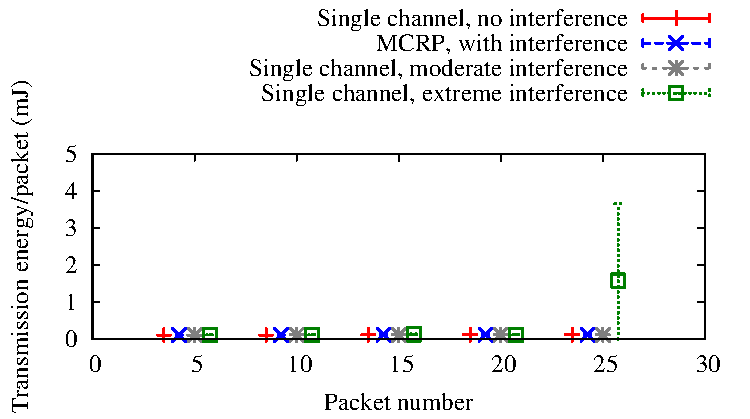
\includegraphics[width=0.45\textwidth]{figures/2EnergyPerPkt.pdf}}                
\subfigure[Node 5 energy consumption]{\label{fig:5perPkt}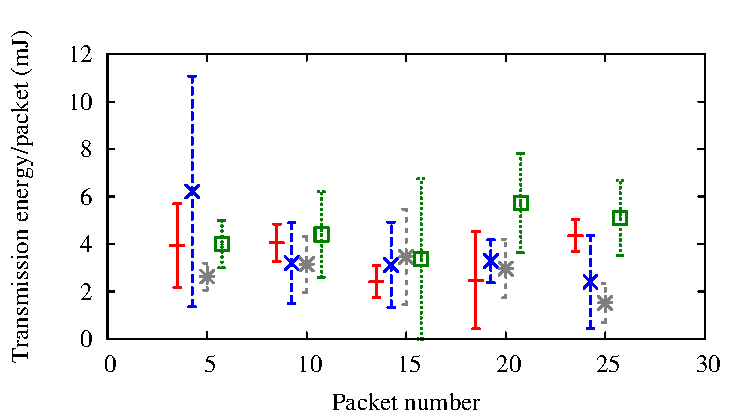
\includegraphics[width=0.45\textwidth]{figures/5EnergyPerPkt.pdf}}
\subfigure[Node 15 energy consumption]{\label{fig:fperPkt}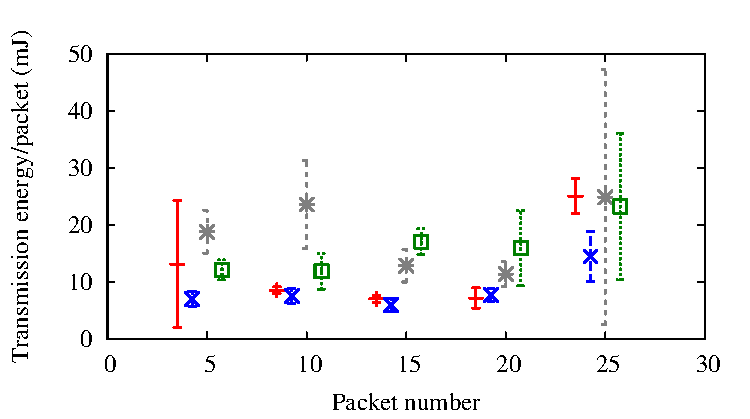
\includegraphics[width=0.45\textwidth]{figures/fEnergyPerPkt.pdf}}
\caption{Comparison of energy consumption per packet for node 2, 5 and 15}
\label{fig:energyPerPkt}
\end{figure}

Figure \ref{fig:energyPerPkt} shows the transmission energy per packet for node 2, 5 and 15. From the figure, it can be concluded that less transmission energy is used when there is less number of hops. However, in a large scale network, the number of hops cannot be reduced as not all nodes would be in the range or directly connected to the destination node. Thus, the node's next hop should be selected carefully to avoid nodes that have higher interference rate.

Node 2 energy consumption in Figure \ref{fig:2perPkt} for the 5th, 10th, 15th, 20th and 25th packet consumed approximately similar energy in all cases. As node 2 is one hop to the destination (LPBR), it was not affected by the interference except for a slight variation in the single channel with extreme interference case for packet 25. Node 3 gives similar result to node 2 as it is also one hop to the LPBR. 

Figure \ref{fig:5perPkt} and Figure \ref{fig:fperPkt} show higher values of energy that a packet requires from the sender (node 5 and 15) to LPBR through 2 and 3 hops. 
This is because of the interference near to the nodes. The nodes are unable to detect the exact wake-up time for the nodes thus, the nodes have to transmit in a longer period to ensure the packet gets transmitted. In the one hop graph, the energy can be kept at minimum because the LPBR is always awake to accept packet as it is fully powered unlike the other nodes that have to switch the radio off when there are no transmissions and receptions taking place to save the energy.

In both graphs, MCRP shows approximately similar transmission energy consumption to the base case. The transmission energy for a single channel with moderate and extreme interference is slightly higher compared to MCRP in 2 hops. In 3 hops, the energy per packet in the single channel with moderate and extreme interference are much higher than the energy used by the base case and MCRP. This shows that the energy per packet depends on the number of hops and the interference that affect the routes. Multichannel helps to mitigate the effect of interference, thus reducing the transmission energy taken to send a packet.

\subsubsection{Energy Over Time Performance}

\begin{figure}
\centering
\subfigure[Node 2 energy consumption]{\label{fig:2total}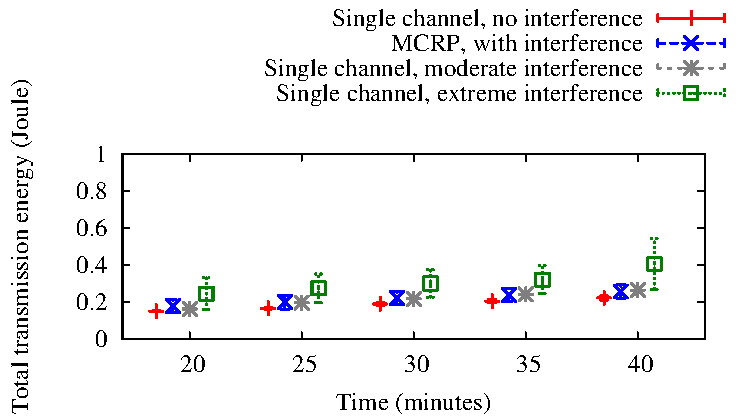
\includegraphics[width=0.45\textwidth]{figures/2Energy.pdf}}      
\subfigure[Node 5 energy consumption]{\label{fig:5total}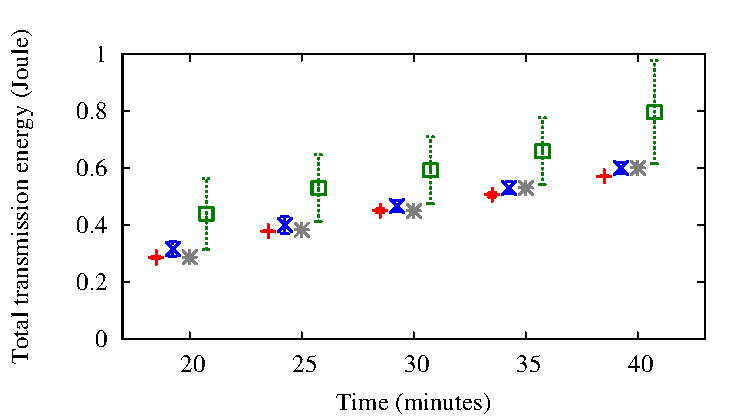
\includegraphics[width=0.45\textwidth]{figures/5Energy.pdf}}          
\subfigure[Node 15 energy consumption]{\label{fig:ftotal}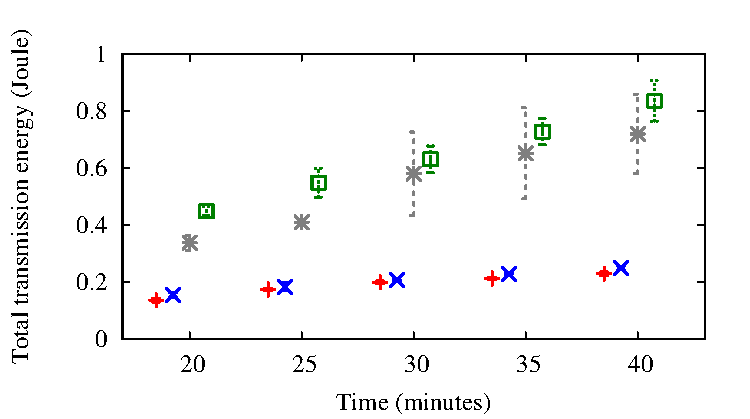
\includegraphics[width=0.45\textwidth]{figures/fEnergy.pdf}}
\caption{Comparison of total energy consumption for node 2, 5 and 15}
\label{fig:energyTotal}
\end{figure}

Figure \ref{fig:energyTotal} shows the graphs of the three nodes total energy consumption that the nodes took to send 25 packets (approximately 40 minutes) including retransmissions and control packets energy. Figure \ref{fig:2total} shows node 2 energy consumption where it can be seen that in all cases, the total energy taken are approximately similar with a small increase over time. The single channel with extreme interference case however, requires more energy consumption than in other cases. Figure \ref{fig:5total} shows higher increase in energy usage over time in all cases. The reason for this is because node 5 has 2 other nodes that are using it as a forwarder. Node 5 (2 hops) uses higher energy when forwarding packet to LPBR compared to node 2 (1 hop). Figure \ref{fig:ftotal} shows lower energy consumption for node 15 compared to node 5 because node 15 does not act as a forwarder.

\begin{figure}
\centering
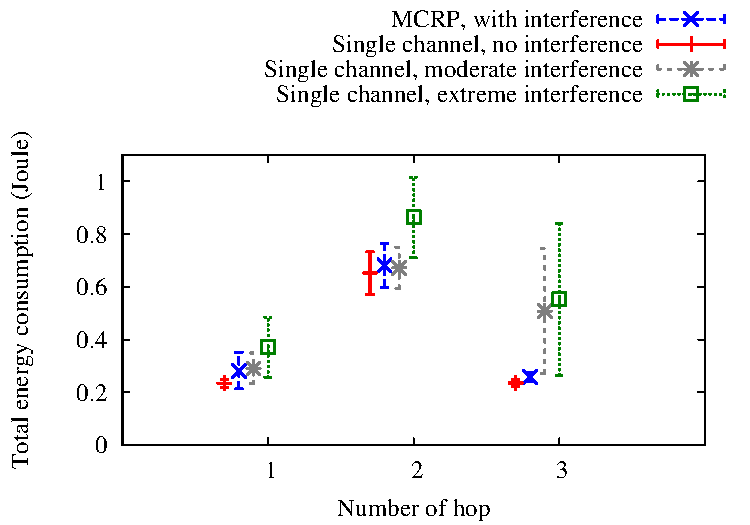
\includegraphics[width=0.45\textwidth]{figures/totalEnergy.pdf}
\caption{Simulation nodes total energy}
\label{fig:allNodesEnergy}
\end{figure}

Figure \ref{fig:allNodesEnergy} shows the total energy consumption for all nodes in the simulation. Node 2 and node 3 are one hop to LPBR, nodes 4-7 are 2 hops, and other nodes are 3 hops away. For most nodes, the energy consumption is slightly improved when using MCRP than a single channel with interference. This improvement can be clearly seen in the 2 hops nodes as these nodes use more energy during interference for retransmissions. If the retransmissions fail, the packet is dropped and the energy used during the retransmissions is wasted. The total energy consumption graph shows all energy from the packet transmission including failed packet energy.

\subsubsection{Forwarding Energy Analysis}

\begin{figure}
\centering
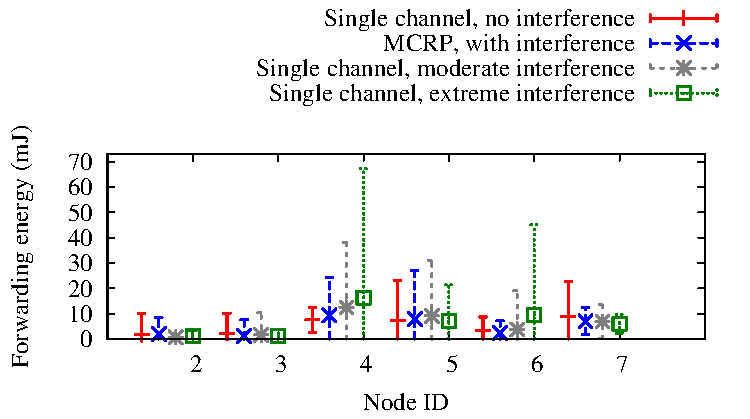
\includegraphics[width=0.45\textwidth]{figures/fwdEnergy.pdf}
\caption{Simulation nodes forwarding energy}
\label{fig:allNodesFwdEnergy}
\end{figure}

Figure \ref{fig:allNodesFwdEnergy} shows the energy used in forwarding packets for nodes 2-7. The other nodes in the simulation do not forward packets. Node 2 and 3 use less energy than nodes 4-7 as the nodes only need to check if the channel is being use by the other node before it can forward to the LPBR. LPBR waits for incoming packet thus the nodes could send the packet with less waiting time as LPBR radio is always on. Based on the simulation layout in Figure \ref{fig_simulation}, node 4 and 5 forward packets to node 2 while node 6 and 7 to node 3 as their next hop. Node 4-7 use higher energy than node 2 and 3 in forwarding packets as the nodes have more packets (from the children) to be forwarded. In order to be able to forward the packets, the nodes have to be awake for longer time and ensure the next hop is also awake and ready to accept the packets. Thus forwarding takes more energy consumption than an end to end packet transmission. By increasing the number of nodes thus children, the nodes will use more energy in order to forward the packets. The forwarding energy consumption contributes to the most energy used by the nodes. MCRP helps to reduce the energy consumption which can be seen in node 4 and 6 results than in a single channel. In the base case, the energy consumption varies as the nodes are interfering with each other even without external interference during transmissions.

%/////

%This chapter presents the estimated energy consumption calculation. Contiki implemented Powertrace which is a software based energy estimation. MCRP uses Powertrace which tracks the duty cycle and uses the values to measure the estimated energy consumption. 
The simulation results showed that MCRP consumes less energy than in other cases when there is interference as the effect of multichannel. In order to increase the energy efficiency thus network lifetime, MCRP needs to reconstruct the topology based on the energy consumption, residual energy of the nodes and the link conditions gradually to avoid breaking any current connectivity.
%The next chapter explains MCRP tree optimisation in details.

\section{Energy-based Tree Reconfiguration}
\label{OptimalTree}

RPL uses ETX which is the expected number of transmissions to reflect the link reliability and the expected latency on the channel. The ETX value is calculated by the node in selecting the next hop route. In order to find the optimal tree, it is assumed that RPL has selected the best routes and MCRP further improved the selected paths by switching to better channels for the transmissions. However, the current best paths do not take into account the nodes residual energy. This could drain the battery of certain nodes quicker than other nodes. RPL can reconstruct the tree as the result of MCRP. The routes might have better reliability in the new channel than it was previously.

%/////Explanation of ETX - The distance from the node relative to the other nodes with respect to the root is called rank. The rank increases away from the root and decreases when it is nearer to the root. Rank is used to avoid routing loop in the topology as the node’s position relative to the other nodes is known.////kind of like Dijkstra

\subsection{Details of Optimal Tree Reconfiguration}

In order to maximise the network lifetime, MCRP has to consider swapping the paths. The optimal tree swapping has to take into account the number of children and descendants to balance the energy consumption in the network based on the residual energy of the nodes. 
The proposal aims to find the tree that could maximise the node with the minimum lifetime. There are three possible solutions that are considered; (a) swap the parent of node $i$, (b) swap the children of node $i$, and (c) swap the descendants of node $i$ that are not the children. However, swapping the parent of the minimum lifetime node does not improve the node lifetime as the number of children and descendants remain same. Thus, only option (b) and (c) are further investigated.  

\begin{equation}
l_i = \frac{e_i}{{(d_i + 1)t_{ip(i)} + \sum_{j \in c(i)} (d_j + 1)t_{ji}}}
\label{optimalEq}
\end{equation}

Equation \ref{optimalEq} shows MCRP optimal tree calculation where $l_i$ is the node $i$ current lifetime based on the node's remaining energy $e_i$ (in percentage), $d_i$ is the number of descendants, $t_{ij}$ represents the number of transmissions on average from node $i$ to node $j$, $p(i)$ refers to the parent of $i$ and $c(i)$ is node $i$ set of children.

\begin{algorithm}
\caption{Pseudo-code for MCRP optimal tree algorithm}
\label{mcrp_algo}
\begin{algorithmic}[]
\\\textbf{Notations}
%\\$e_i$ is the node battery power
\\$l_i$ is the node lifetime
\\$c_i$ is the number of node $i$ children
\\$d_i$ is the number of node $i$ descendants
%\\$t_{ij}$ is the number of transmissions on average from $i$ to $j$
%\\$p(i)$ is the parent of node $i$
%\\$c(i)$ is the set of node $i$ children
\\\textbf{Pseudo-code}
\\Form tree based on MCRP
\\Update battery level for all nodes
\\Update all nodes $l_i$, $c_i$, $d_i$
\\minimum $\leftarrow$ 0
\\previousSwapNode $\leftarrow$ 0 
  \While{node $\neq$ previousSwapNode}
    \State Find node with minimum $l_i$
    \State List all potential $c_i$ and $d_i$ swap
	\If{$c_i$ and $d_i$ swap $l_i$ $>$ minimum} %to avoid cycle
		\State Recalculate all nodes $l_i$
		\If{all new nodes $l_i$ $>$ minimum}
			\State Update tree
			\State New tree is optimal
		\Else
			\State Revert to previous optimal tree
		\EndIf
			\State previousSwapNode $\leftarrow$ node
	\Else
		\State Current tree is optimal
	\EndIf
  \EndWhile
\end{algorithmic}
\end{algorithm}

Algorithm \ref{mcrp_algo} describes the swapping processes based on the nodes lifetime calculated from Equation \ref{optimalEq}. It considers all available paths between the nodes and shows all potential topologies before deciding on the optimal tree.
It is assumed that all nodes residual energy and the paths are known. Both the nodes battery and the link conditions can deteriorate over time. However, it is assumed that the current selected paths are the favourable routes selected by the MCRP, thus, only the battery level of the nodes is the variable. The topology is changed accordingly where the nodes that have the minimum value is selected to balance the network in term of the battery, link conditions and the number of children and descendants. The network is considered as balanced in term of the lifetime which means, the number of nodes and descendants connected might not be fairly distributed as the battery level vary in each node.

\subsection{Illustrative Example}

Figure \ref{fig:ot} is an illustrative example to explain the algorithm proposed. Assumed that the tree formed in Figure \ref{fig:ot-1} is the current optimal tree after running MCRP processes. Each node is labelled with the battery level, represented in percentage for simplicity. It can also be represented in volts or Joules. The lines between the nodes represent routes in different channels where dotted lines are the potential routes and the solid lines are the current routes. The values represent the link conditions in terms of the number of successful expected transmission between the two nodes. The values of the links are the expected transmission taken only for the upwards route as the links downwards could have different values due to the different transmission and reception channels on each node thus different link quality. 
%The main reason for this difference is due to the two hops algorithm implemented in MCRP. 
The transmission and reception channels of a node cannot be the same to avoid interference with nearby nodes.
%Figure \ref{fig:graphTree1-2} is the simplified graph of Figure \ref{fig:graphTree1} where the nodes are (labelled?) with their lifetime calculated based on the paths (solid lines) and the potential edges are the link condition values of the node pair.

The figure shows that node 2 has the most descendants which consequently reduce the node lifetime as it has to forward more packets than any other nodes. Initially, the topology is formed based on the least value on the paths. In order to optimise the tree, the overall network lifetime is considered where paths that are not the minimum could be chosen as the route as it prolongs the overall functionality of the network. In this example, node 2 has the minimum lifetime. It can be maximised through swaps. 

There are several potential swaps to improve node 2 lifetime that includes both the children which are node 5 and 6, and the children of children, node 7 and 8. Figure \ref{fig:ot-2} shows node 5 swaps to node 4 instead of its initial node 2 and the network lifetime is calculated. Node 2 lifetime is improved, however, node 1 has a lower lifetime than the initial minimum value as the result of swapping. Node 1 now has 5 descendants while node 2 only has one when it initially had 4. In order to reduce the number of unnecessary swap, once the maximum minimum lifetime is found, all nodes lifetime values are checked to ensure that they have higher lifetime than the initial minimum lifetime regardless of the maximising the minimum node to avoid endless cycle of swaps. While the swap done by node 5 improves node 2 lifetime, node 1 lifetime deteriorates to a value lower than the minimum. The network reverts to the previous topology that is better than the new swap. Node 5 tries and swaps to node 6, then node 6 swaps to node 8. However, the potential topology is not improved. Node 2 then swaps its descendants node 7 and 8.

When node 7 is swaps to node 4 instead of node 5, the tree is improved. It can be seen in Figure \ref{fig:ot-3} that the tree is more balanced and node 2 lifetime is prolonged. As the result of swapping, node 4 lifetime is reduced as the path from node 7 to node 4 is not the smallest path value. The tree is updated as the current optimal tree. It is not yet the final optimal tree because node 8, which is another node 2 descendant has not been checked. If node 8 swap does not improve the tree, the swap from node 7 is chosen as the final optimal tree. 
Another potential swap is shown in Figure \ref{fig:ot-4} where node 8 is connected to node 6 instead of node 5. In both cases, node 2 lifetime is maximised and all nodes lifetime are above the minimum value. The tree in Figure \ref{fig:ot-3} is selected as the final optimal tree in maximising node 2 lifetime. Further investigations are required in order to decide the criteria on an optimal tree when there are several good topologies to be selected. 

Node 1 is then selected as the minimum lifetime as node 2 cannot be selected again to avoid unnecessary repetition. Optimal tree from the potential swaps for node 1 is not found thus the tree is said to be optimal. In the algorithm, the same node cannot swap again right after its previous swap. This is done to avoid oscillation which would produce similar result. The node however, could swaps in the next round as the other node swap would have changed the topology.

The swaps are assumed to happen once until the network stops functioning, thus the overheads are negligible. The swapping calculations and decisions are made by the LPBR due to sensors limitations and constraints. LPBR informs the specific nodes of the final swapping if it needs to take place. In term of energy cost, the cost is negligible as the swaps are infrequent and being controlled by the LPBR.

\begin{figure}
\centering
\subfigure[Initial tree]{\label{fig:ot-1}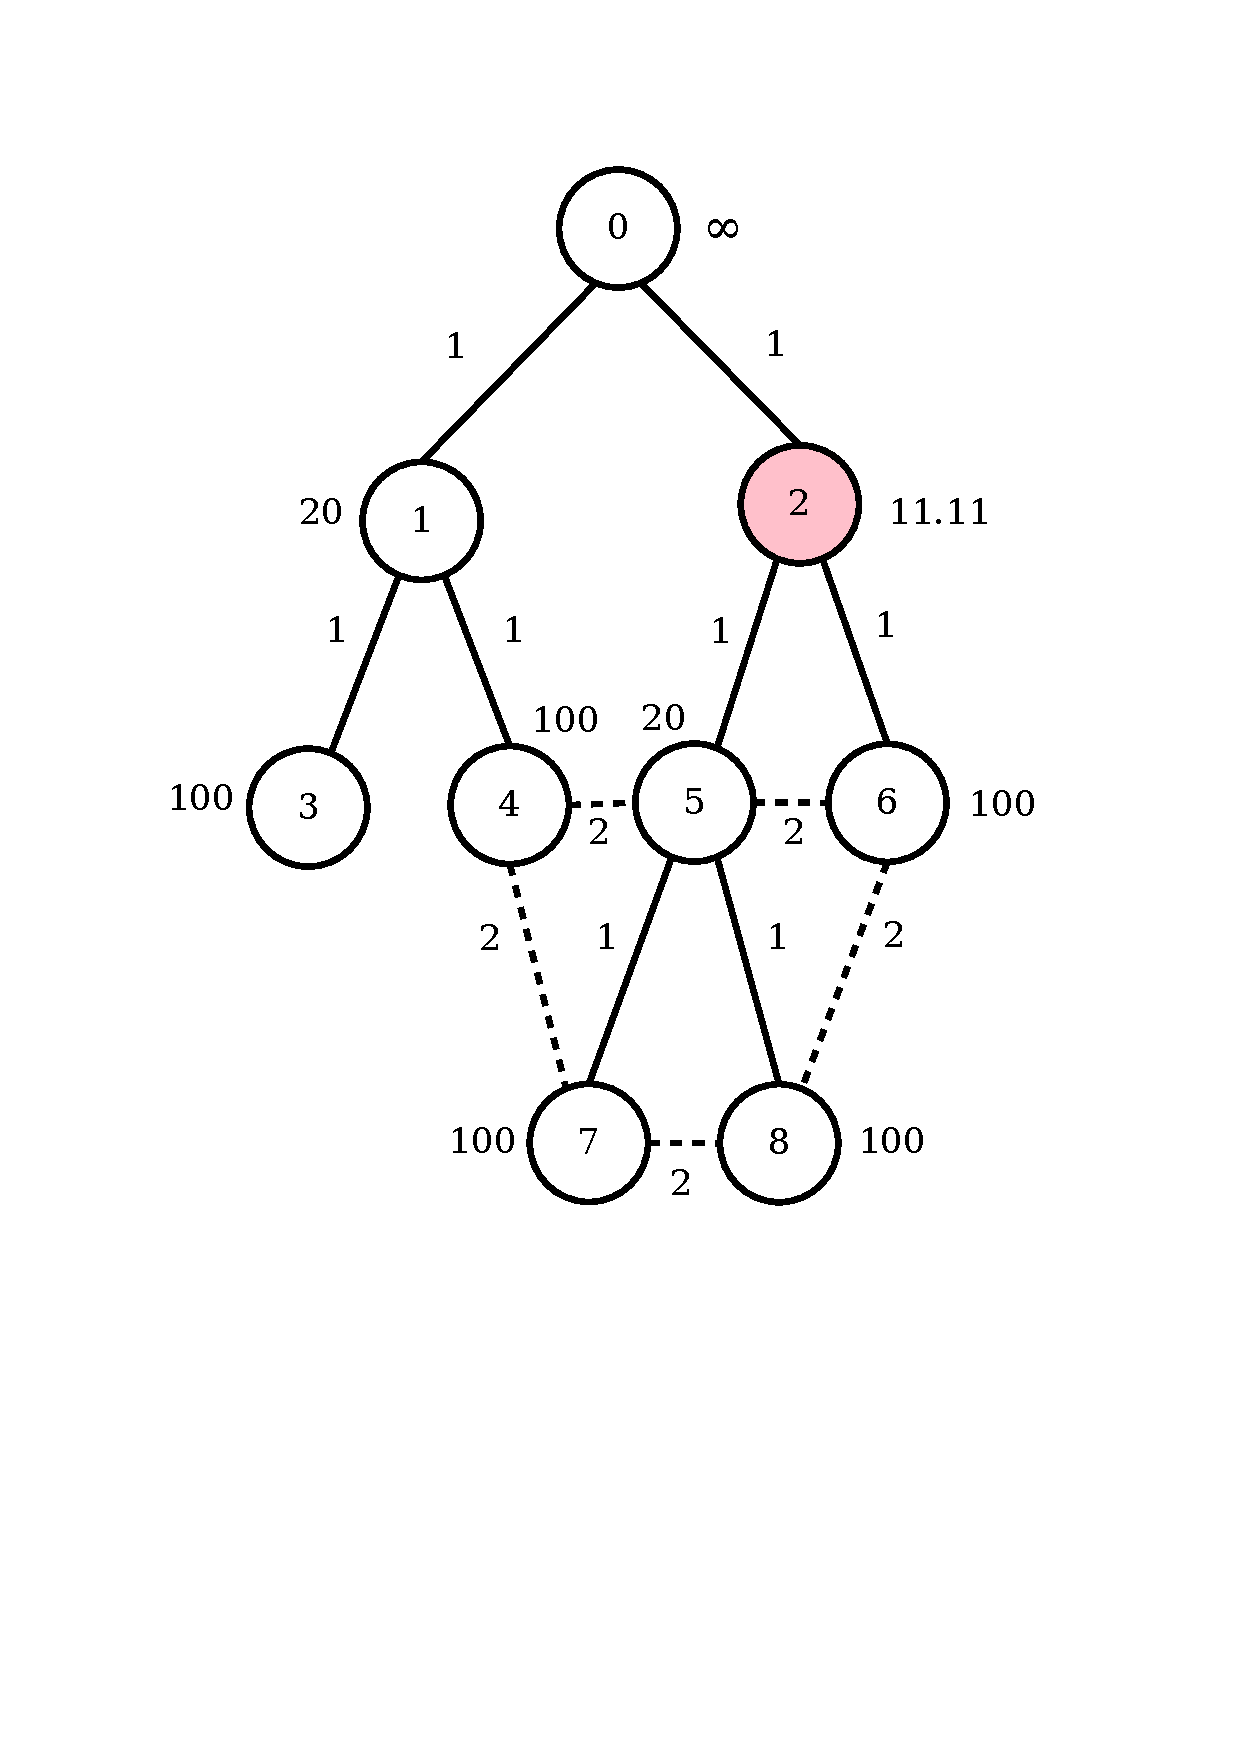
\includegraphics[page=1, trim=2cm 9cm 2cm 2cm, clip=true, totalheight=0.19\textheight]
{figures/ot1.pdf}}        
%\hfill        
\subfigure[Node 5 swaps to node 4]{\label{fig:ot-2}\includegraphics[page=2, trim=2cm 9cm 2cm 2cm, clip=true, totalheight=0.19\textheight]
{figures/ot1.pdf}}
%\hfill        
\subfigure[Node 7 swaps to node 4]{\label{fig:ot-3}\includegraphics[page=3, trim=2cm 9cm 2cm 2cm, clip=true, totalheight=0.19\textheight]
{figures/ot1.pdf}}
%\hfill        
\subfigure[Node 8 swaps to node 6]{\label{fig:ot-4}\includegraphics[page=4, trim=2cm 9cm 2cm 2cm, clip=true, totalheight=0.19\textheight]
{figures/ot1.pdf}}
\caption{Graph of the bidirectional paths in a WSN}
\label{fig:ot}
\end{figure}
\section{Performance Evaluation}
\label{PerformanceEvaluation}

This section describes the evaluation of the following performance metrics: (a) the average number of switches to form the optimal tree and (b) the impact of swapping on the network lifetime.  

%\subsection{MCRP Results}

\subsection{Simulation Setup}

The optimal tree algorithm is simulated in C. The number of sensors considered is between 10 to 500 and each node is randomly assigned an initial energy between 50\% to 100\%. The link conditions are also randomly assigned the value between 1 to 10 where smaller number indicates better link condition as it requires smaller number of retransmissions. In this setup, the channels are fixed, assuming that the current channels that the nodes are listening and transmitting on, are the best selected channels from the previous MCRP processes. RPL builds the initial tree based on the ETX value which is then further improved by MCRP. In order to avoid all the nodes from directly connecting to the LPBR, each node could route to a minimum of $1/10$ and $1/30$ of the total number of nodes. %As each path is bi-directional,  
This allows the node to have alternative parents (thus paths) for the swapping processes and hops to reach the LPBR. The node is not necessarily connected to all $1/10$ and $1/30$ nodes. The paths between the nodes are selected based on the RPL and MCRP processes. These values are selected in the case where (a) the nodes are closely together ($1/10$), and (b) the nodes are spread out with minimum connections to the other nodes available ($1/30$). 

\subsection{Simulation Results}
\subsubsection{Average Number of Switches}

\begin{figure}
\centering
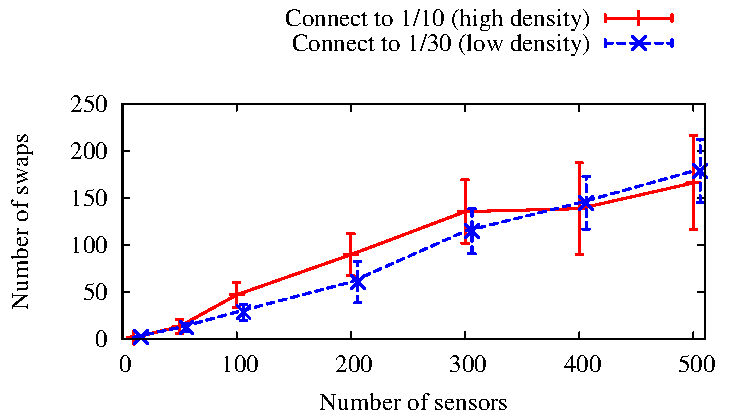
\includegraphics[width=0.45\textwidth]{figures/swaps.pdf}
\caption{Average number of swaps}
\label{fig:aveSwaps}
\end{figure}

Figure \ref{fig:aveSwaps} shows the standard deviation and average number of swaps using MCRP optimal tree algorithm. 
The standard deviation on the x axis is slightly shifted to avoid overlapping.
It can be observed that there are more swaps on average when there are more sensors in the network in both connection cases. However, nodes that could route to $1/10$ of the total sensors showed slightly higher number of swaps than in the $1/30$ connection. The reason for this is because in $1/10$ connection, it has more neighbours, hence many potential parents to select. 
%In term of time taken for swapping, it takes slightly longer to finalise the swap when the network size increases. 

In a smaller network, the sensors are limited by the number of potential parents. This prevents the nodes from swapping as the potential parents might not have any improvement. This can be seen from the number of swaps in a 50 sensors network where the average number of swaps is less than 10. This is because each node has 5 (in $1/10$) and 2 (in $1/30$) potential parents to select from unlike in the 500 sensors network which each has 50 and 17 potential parents. However, as there are more sensors, it takes longer to find the best parents as the swaps will consider all nodes that are within the range.

This experiment does not reflect the condition in the real world where the sensors could be scattered with more or less available range to the other nodes depending on the application; which means more nodes can directly be connected to the LPBR without hops in between. This however, represents a reasonable connection between the nodes to allow swapping and alternative nodes if the current forwarding nodes values are at a minimum for the experiment.

\subsubsection{Impact On The Network Lifetime}

\begin{figure}
\centering
%\subfigure[10 nodes]{\label{fig:10maxmin}\includegraphics[width=0.78\textwidth]{treeFigures/maxmin10.pdf}}                
\subfigure[Connect to 1/10 of total sensors]{\label{fig:1-10}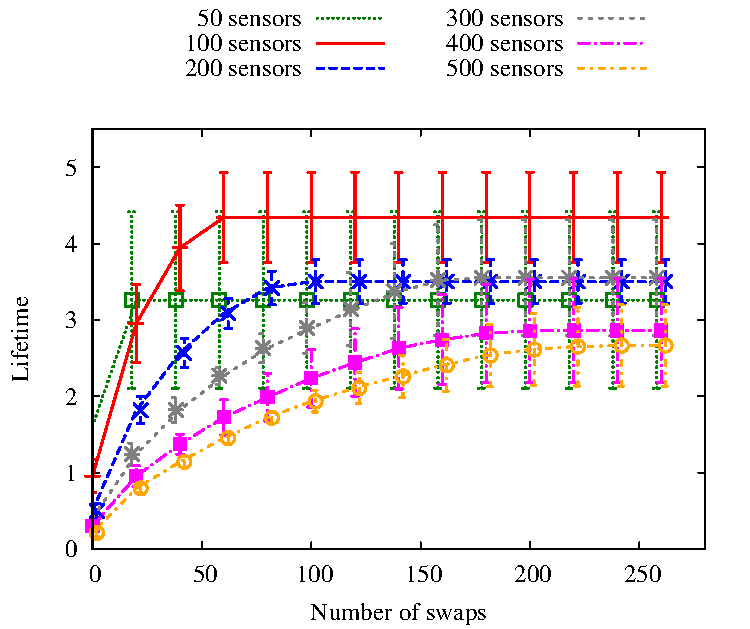
\includegraphics[width=0.45\textwidth]{figures/lifetime1.pdf}}
\subfigure[Connect to 1/30 of total sensors]{\label{fig:1-30}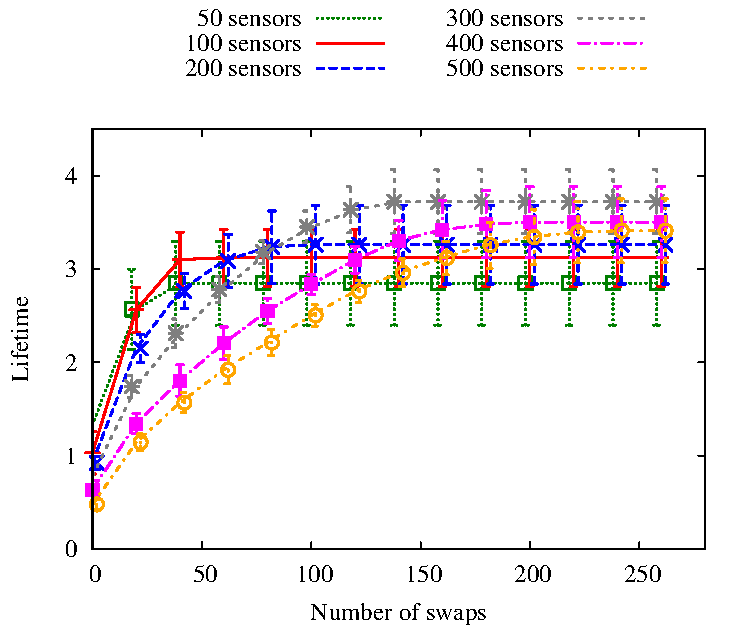
\includegraphics[width=0.45\textwidth]{figures/lifetime3.pdf}}
\caption{Comparison of the number of swaps and lifetime in different network scale}
\label{fig:maxmin}
\end{figure}


Figure \ref{fig:maxmin} shows the improvement in the node thus network lifetime by maximising the minimum and the number of swaps required in 10 runs in 6 networks with 50, 100, 200, 300, 400 and 500 sensors with different degree of connection. 
The standard deviation on the x axis is slightly shifted to prevent the error bars from overlapping.
It is observed that the node lifetime decreases with an increase in the number of sensors in the network. The reason for this is in a larger network, there are a higher number of descendants and each connection has its own path values. By taking into account these variables, the number of nodes affect the whole network lifetime. While a higher number of nodes allow more alternative routes, it also consumes more energy as there are more connected nodes. Smaller network however, has limited number of possible swaps which does not improve the network lifetime.

Figure \ref{fig:1-10} shows the number of swaps and the lifetime when the nodes are connected to $1/10$ of the total nodes in the network. 
In the 50 nodes network, the number of swaps is less than 10 before it reaches the maximum lifetime for the whole network. 
As the number of sensors in the network increase, it takes more swaps before the tree is optimal. 
In the 200 nodes network, the number of swaps is around 100 swaps and the lifetime is improved from the minimum of 0.5\% to 3.1\%. In 500 nodes network, it takes more swaps, around 200 swaps for the lifetime to be maximised from 0.3\% to 2.5\%. 

Figure \ref{fig:1-30} shows similar improvement in the $1/30$ connection case. However, it can be seen that the maximum lifetime values in the figure for 100 sensors network is slightly less than in Figure \ref{fig:1-10}. This is because the networks have lesser potential parents and paths to select from. The tree is limited by the number of connections. The other large networks have similar maximum lifetime values in both figures.

\begin{figure}
\centering
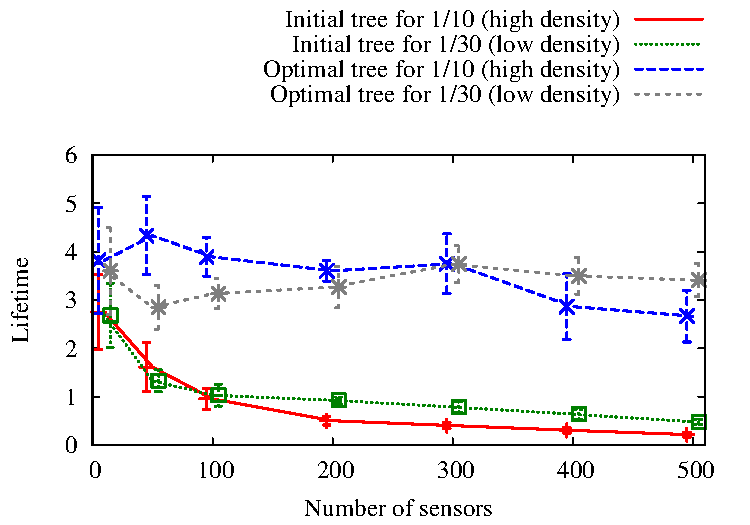
\includegraphics[width=0.45\textwidth]{figures/maxmin.pdf}
\caption{Lifetime of MCRP optimal tree}
\label{fig:nodes-maxmin}
\end{figure}

Figure \ref{fig:nodes-maxmin} shows the comparison between the initial and optimal tree in both cases. The standard deviation on the x axis is slightly shifted to the left and right to prevent the error bars from overlapping. MCRP swapping prolongs the network lifetime which shows an increase from the initial lifetime. Smaller networks have high initial lifetime values compared to larger networks. However, larger networks have better lifetime improvement than the slight improvement in smaller networks.

In the initial trees, it can be seen that when there are more sensors in the network, the lifetime values are decreasing. This shows the importance of finding the optimal tree as the results showed that the lifetime can be improved by approximately 3\% when initially, in all networks, the minimum sensors have less than 1\% lifetime. The increase enables the network to remain functional slightly longer than initially. 
\section{Conclusion}
\label{Conclusion}

In this paper, a two step optimisation approaches were presented that reduce the effect of interference by implementing MCRP, a multichannel cross-layer routing protocol, and maximise the network lifetime by reconfiguring the topology to find the optimal tree. 
MCRP shows high packet reception rate in simulations and hardware results. In addition, MCRP reduces the energy consumption by an average of 6 times during communications as the effect of multichannel.
%in addition to the reduced energy consumptions during communications as the effect of multichannel.  
The energy-based tree reconfiguration is proposed to further improve the multichannel network by considering the energy level of each sensor. 
%The sensors are balanced in term of the ability to route packets based on the residual energy available.
%The sensors residual energy are balanced
%The equation and algorithm used in finding the optimal tree are explained. 
It is aimed to enable the network to be fully functional for a longer period of time by maximising the minimum sensor energy level and enable the sensors to have similar lifetime.
%through topology reconstruction. 
The results showed an increase in the network lifetime by 8.3 times more for the optimal tree compared to the initial tree in a 500 nodes system.

% use section* for acknowledgment
\section*{Acknowledgment}


The authors would like to thank...

\label{references}
%\nocite{*}
\bibliography{main}
\bibliographystyle{IEEEtran}
%\bibliographystyle{plain}


%\subsection{Subsection Heading Here}
%Subsection text here.

%\subsubsection{Subsubsection Heading Here}
%Subsubsection text here.


% An example of a floating figure using the graphicx package.
% Note that \label must occur AFTER (or within) \caption.
% For figures, \caption should occur after the \includegraphics.
% Note that IEEEtran v1.7 and later has special internal code that
% is designed to preserve the operation of \label within \caption
% even when the captionsoff option is in effect. However, because
% of issues like this, it may be the safest practice to put all your
% \label just after \caption rather than within \caption{}.
%
% Reminder: the "draftcls" or "draftclsnofoot", not "draft", class
% option should be used if it is desired that the figures are to be
% displayed while in draft mode.
%
%\begin{figure}[!t]
%\centering
%\includegraphics[width=2.5in]{myfigure}
% where an .eps filename suffix will be assumed under latex, 
% and a .pdf suffix will be assumed for pdflatex; or what has been declared
% via \DeclareGraphicsExtensions.
%\caption{Simulation results for the network.}
%\label{fig_sim}
%\end{figure}

% Note that the IEEE typically puts floats only at the top, even when this
% results in a large percentage of a column being occupied by floats.


% An example of a double column floating figure using two subfigures.
% (The subfig.sty package must be loaded for this to work.)
% The subfigure \label commands are set within each subfloat command,
% and the \label for the overall figure must come after \caption.
% \hfil is used as a separator to get equal spacing.
% Watch out that the combined width of all the subfigures on a 
% line do not exceed the text width or a line break will occur.
%
%\begin{figure*}[!t]
%\centering
%\subfloat[Case I]{\includegraphics[width=2.5in]{box}%
%\label{fig_first_case}}
%\hfil
%\subfloat[Case II]{\includegraphics[width=2.5in]{box}%
%\label{fig_second_case}}
%\caption{Simulation results for the network.}
%\label{fig_sim}
%\end{figure*}
%
% Note that often IEEE papers with subfigures do not employ subfigure
% captions (using the optional argument to \subfloat[]), but instead will
% reference/describe all of them (a), (b), etc., within the main caption.
% Be aware that for subfig.sty to generate the (a), (b), etc., subfigure
% labels, the optional argument to \subfloat must be present. If a
% subcaption is not desired, just leave its contents blank,
% e.g., \subfloat[].


% An example of a floating table. Note that, for IEEE style tables, the
% \caption command should come BEFORE the table and, given that table
% captions serve much like titles, are usually capitalized except for words
% such as a, an, and, as, at, but, by, for, in, nor, of, on, or, the, to
% and up, which are usually not capitalized unless they are the first or
% last word of the caption. Table text will default to \footnotesize as
% the IEEE normally uses this smaller font for tables.
% The \label must come after \caption as always.
%
%\begin{table}[!t]
%% increase table row spacing, adjust to taste
%\renewcommand{\arraystretch}{1.3}
% if using array.sty, it might be a good idea to tweak the value of
% \extrarowheight as needed to properly center the text within the cells
%\caption{An Example of a Table}
%\label{table_example}
%\centering
%% Some packages, such as MDW tools, offer better commands for making tables
%% than the plain LaTeX2e tabular which is used here.
%\begin{tabular}{|c||c|}
%\hline
%One & Two\\
%\hline
%Three & Four\\
%\hline
%\end{tabular}
%\end{table}


% Note that the IEEE does not put floats in the very first column
% - or typically anywhere on the first page for that matter. Also,
% in-text middle ("here") positioning is typically not used, but it
% is allowed and encouraged for Computer Society conferences (but
% not Computer Society journals). Most IEEE journals/conferences use
% top floats exclusively. 
% Note that, LaTeX2e, unlike IEEE journals/conferences, places
% footnotes above bottom floats. This can be corrected via the
% \fnbelowfloat command of the stfloats package.


%\appendices
%\section{Proof of the First Zonklar Equation}
%Appendix one text goes here.

% you can choose not to have a title for an appendix
% if you want by leaving the argument blank
%\section{}
%Appendix two text goes here.



% Can use something like this to put references on a page
% by themselves when using endfloat and the captionsoff option.
\ifCLASSOPTIONcaptionsoff
  \newpage
\fi



% trigger a \newpage just before the given reference
% number - used to balance the columns on the last page
% adjust value as needed - may need to be readjusted if
% the document is modified later
%\IEEEtriggeratref{8}
% The "triggered" command can be changed if desired:
%\IEEEtriggercmd{\enlargethispage{-5in}}

% references section

% can use a bibliography generated by BibTeX as a .bbl file
% BibTeX documentation can be easily obtained at:
% http://mirror.ctan.org/biblio/bibtex/contrib/doc/
% The IEEEtran BibTeX style support page is at:
% http://www.michaelshell.org/tex/ieeetran/bibtex/
%\bibliographystyle{IEEEtran}
% argument is your BibTeX string definitions and bibliography database(s)
%\bibliography{IEEEabrv,../bib/paper}
%
% <OR> manually copy in the resultant .bbl file
% set second argument of \begin to the number of references
% (used to reserve space for the reference number labels box)

%\begin{thebibliography}{1}

%\bibitem{IEEEhowto:kopka}
%H.~Kopka and P.~W. Daly, \emph{A Guide to \LaTeX}, 3rd~ed.\hskip 1em plus
%  0.5em minus 0.4em\relax Harlow, England: Addison-Wesley, 1999.

%\end{thebibliography}

% biography section
% 
% If you have an EPS/PDF photo (graphicx package needed) extra braces are
% needed around the contents of the optional argument to biography to prevent
% the LaTeX parser from getting confused when it sees the complicated
% \includegraphics command within an optional argument. (You could create
% your own custom macro containing the \includegraphics command to make things
% simpler here.)
%\begin{IEEEbiography}[{\includegraphics[width=1in,height=1.25in,clip,keepaspectratio]{mshell}}]{Michael Shell}
% or if you just want to reserve a space for a photo:

\begin{IEEEbiography}{Michael Shell}
Biography text here.
\end{IEEEbiography}

% if you will not have a photo at all:
\begin{IEEEbiographynophoto}{John Doe}
Biography text here.
\end{IEEEbiographynophoto}

% insert where needed to balance the two columns on the last page with
% biographies
%\newpage

\begin{IEEEbiographynophoto}{Jane Doe}
Biography text here.
\end{IEEEbiographynophoto}

% You can push biographies down or up by placing
% a \vfill before or after them. The appropriate
% use of \vfill depends on what kind of text is
% on the last page and whether or not the columns
% are being equalized.

%\vfill

% Can be used to pull up biographies so that the bottom of the last one
% is flush with the other column.
%\enlargethispage{-5in}



% that's all folks
\end{document}


